\documentclass[runningheads]{llncs}
\usepackage[T1]{fontenc}

% define lightgray
\usepackage[table]{xcolor}

\usepackage{booktabs}
\usepackage[square,sort,comma,numbers]{natbib}
\usepackage[pdfstartview=XYZ,
bookmarks=true,
colorlinks=true,
linkcolor=blue,
urlcolor=blue,
citecolor=blue,
pdftex,
bookmarks=true,
linktocpage=true, % makes the page number as hyperlink in table of content
hyperindex=true
]{hyperref}

\usepackage{orcidlink} % orcidlink
\usepackage{marvosym} %letter symbol
\usepackage{rotating} % Rotating table
\usepackage{subcaption}
\usepackage{graphicx}

\usepackage{amsmath}

\newcommand{\myvec}[1]{\mathbf{#1}}

\title{Comparing efficiency, utility, and privacy between synthetic data packages and methods}
\titlerunning{Comparing efficiency, utility, and privacy}

\author{Jörg Drechsler\inst{1 (\text{\Letter})} \and
Jonathan Latner\inst{1 \orcidlink{0000-0002-1825-0097}} \and
Marcel Neunhoeffer\inst{1 \orcidlink{0000-0002-9137-5785}}}

\authorrunning{Drechsler et al., \the\year}

\institute{Institute for Employment Research, Nuremberg, Germany
\email{\{joerg.drechsler,jonathan.latner,marcel.neunhoeffer\}@iab.de}}

\begin{document}

\maketitle              % typeset the header of the contribution

\begin{abstract}
The abstract should briefly summarize the contents of the paper in
150--250 words.

\keywords{First keyword  \and Second keyword \and Another keyword.}
\end{abstract}


\clearpage

\section{Introduction}

The idea of releasing synthetic data instead of actual data is often understood to have begun in the early 1990s \cite{rubin1993statistical,little1993statistical}.  Here, when we refer to data, we are referring to microdata (i.e. one observation per individual unit) as opposed to tabular data (i.e. summary data).  Releasing synthetic data means altering actual data in some way so that the released data do not contain information on a real individual unit (person, firm, etc.) that would reveal information that could be used to identify the unit.  The appeal is that the synthetic data mimic the statistical properties of the original data while maintaining the privacy of individual records.

In its original form, the idea of creating synthetic data is to treat all data not in a sample as missing data from a population to be filled in using multiple imputation.  The missing data are filled in using models fit with the original data to create synthetic data.  Then, multiple random samples of the synthetic data are released to the public to account for variance.  Despite its simplicity, the problem is not only that this approach is model dependent, but also that the synthetic data are not by definition private \cite{reiter2009estimating}.  

Recently, a new generation of synthetic data generators (SDGs) seek to address the weaknesses found in the original approach.  In this paper, we evaluate three SDGs (Synthpop \cite{nowok2016synthpop}, Datasynthesizer \cite{ping2017datasynthesizer}, and CTGAN \cite{ctgan}) using a single data set on four criteria \cite{jordon2022synthetic}: utility, fidelity, privacy, and efficiency, terms that we will define below.  

The results indicate several points that contribute to our understanding of SDGs.  First, one should not confuse a method/model that generates synthetic data with a statistical package containing a given generator.  Even if a given SDG performs poorly on a given criteria, this does not mean that the underlying method is a poor synthesizer or visa versa.  Second, efficiency is a criteria that cannot be ignored.  SDGs that create high quality synthetic data using low-dimensional data often used for testing and evaluation may not scale well as the dimensionality increases.   Third, privacy is a function of the mechanism used by the SDG \cite{jordon2022synthetic}, not the synthetic data created by the SDG.  As such, privacy cannot be evaluated post-hoc.  In contrast to the simplicity of the original idea, and despite decades of progress, the creation of synthetic data remains a complicated process including steps that are either not common knowledge or described in one place.

Section \ref{sec:background} provides a brief introduction to the data synthesis problem, particularly in terms of microdata, and an introduction to the data synthesis methods. Section \ref{sec:study_design} outlines the design of the study, describing the methods and the data used. Section \ref{sec:results} provides the results, and section \ref{sec:conclusion} concludes with directions for future research.

\section{Background}\label{sec:background}

Theoretically, there are multiple goals for generating synthetic data \cite{rubin1993statistical}.  For the survey participants, they could be confident that their data would never be released, which could increase the likelihood not only of more survey respondents, but also more truthful answers.  For the illegitimate user or `snooper,' the value of the data would be eliminated because they could not discover actual, confidential information.  For the researcher, synthetic data can be used to develop code before they have access to the original data.  As a result, high quality synthetic data can increase knowledge creation by allowing more people to use better data.  For the legitimate user, the value of the data would increase not only because the data are easier to access, but also more accurate than the actual data.\footnote{``Experience with these data sets shows that inferences for population estimands involving $Y$ based on the multiply-imputed public-use file appear to be valid, and often, perhaps even typically, $more$ precise [emphasis in original] than the corresponding inferences based on the research file, despite the fact that only entirely synthetic $Y$ vvalues exist in the public-use file and all the real $Y$ values exist in the research file \cite[pg. 466]{rubin1993statistical}.''}  

In reality, most of these goals are problematic.  To our knowledge, there is no evidence that the knowledge that a user's data would never be publicly released either increases the likelihood of survey respondents, nor more truthful answers (XXXX).  Without denying the importance of so-called `intruder' studies that seek to evaluate risk, reports of malicious re-identifications are rare to non-existent \cite{francis_wagner_yyyy}.  In most cases, newspaper or academic articles about re-identifications are not used for malicious intent or profit, but rather to improve data security or awareness of privacy issues.  In addition, while the appeal of synthetic data is to produce more accurate data, low probability events that are essential to the independent and relational variance of variable(s) found in original data are hard to correctly capture in synthetic data, such as observations that are outliers or missing not at random.  

Despite these challenges, for the researcher, the theoretical and realistic goal are the same: synthetic data can make time with original data more efficient and effective.  As a result, even if synthetic data cannot be a replacement for real data, high quality synthetic data can be a valuable tool to accelerate knowledge creation.  

Below, we outline the challenges and compromises one must consider in order to create high quality synthetic data.  There are four key points we wish to make.  First, one must distinguish the method from the package containing a statistical data generator (SDG).  Second, while the literature has long understood the trade-off between utility and privacy \cite{duncan2004database}, this does not distinguish utility from fidelity, which are similar, but not the same.  Third, for reasons we explain below, privacy cannot be evaluated post-hoc, but is rather a component of the SDG.  Finally, though often overlooked, we emphasize the role of efficiency and the curse of dimensionality when creating synthetic data.  

\subsection{Processes, methods, and packages}

In the beginning, the idea of creating synthetic data was a theoretical process \cite{rubin1993statistical}.  To create synthetic data from actual data, all non-respondents in a survey are treated as missing values to be replaced with `imputed' values.  Given a dataset ($D$) with observations ($n$), there is a two-stage process.  First, a model for predicting a given outcome variable ($y$) given a set of background variables ($x$) is trained on the actual data.  Second, values of the original outcome variable are replaced by predicted values of the outcome variable ($y^*$).  This process is then repeated so that all actual values are replaced by imputed values for every variable.  The result is a multiply-imputed synthetic dataset ($D^*$) that contains no values in the actual data, but looks structurally identical to the actual data, not only with respect to mean and variation within a given variable, but also correlations between variables.  Despite the simplicity, implementing the theoretical process is more complicated than the description might suggest.  

One primary question is what method to use.  While the original application may have assumed some sort of parametric estimation using a linear or non-linear model, more recent research borrows from the machine learning literature, including Classification and Regression Trees (CART) \cite{reiter2005using}, Random Forests \cite{caiola2010random}, Support Vector Machines \cite{drechsler2010using}, Bayesian Networks \cite{zhang2017privbayes}, and General Adversarial Networks (GANs) \cite{goodfellow2014generative}, among others.  Evaluations appear to suggest that CART models appear to create synthetic data that are stastically more similar to original data  \cite{little2022comparing,dankar2021fake,drechsler2011empirical}.  

A related question is what package to use.  A statistical package that can be loaded into R or Python or another statistical software program that contains a synthetic data generator (SDG) is not the same thing as the method used by the SDG.  For example, the Python package Synthcity \cite{synthcity} contains multiple types of GANs (CTGAN, AdsGan, etc.) and Bayesian (PrivBayes, Bayesian Network) SDGs.  For SDGs using CART models, options include the Synthpop package \cite{nowok2016synthpop} that implements one variation of CART \cite{reiter2005using} or the MICE package \cite{van2011mice} that implements another \cite{doove2014recursive}.  It is important to distinguish the method from the package in order to reduce confusion when evaluating what SDG is right for what type of research question or data.

\subsection{Utility and fidelity}

While the inverse relationship between utility and privacy is well understood, this assumes a trade-off between utility and privacy that does not distinguish utility from fidelity \cite{jordon2022synthetic}.  Utility and fidelity are sometimes referred to as broad and narrow measures within the single concept of utility \cite{snoke2018general,drechsler2009disclosure}.  While the two are correlated, they are not the same and it is possible for one to change, but not the other.  

Here, utility is defined as the degree to which synthetic data and original data return the same results for a given task or set of tasks \cite{jordon2022synthetic}.  This is most similar to the concept of narrow utility measures \cite{drechsler2009disclosure}.  One example would be to compare and contrast model parameter estimates from original and synthetic data, and their confidence interval overlap (CIO).  A non-parametric example would be to compare and contrast one or two-way frequency of estimates for a single or pair of variable(s), sometimes referred to as a ratio of counts/estimates (ROC/ROE) \cite{little2022comparing}.  

Fidelity is defined as the degree to which synthetic data matches the original data.  One example would be the propensity score.  While the details are described by Snoke et al., \cite{snoke2018general}, the basic idea is a classification problem where the desired result is to not be able to distinguish the original from the synthetic data.  Not surprisingly, there is more than one way to calculate the resulting measure, including Propensity Score Measure Mean Squared Error (pMSE) \cite{woo2009global} and the Kolmogorov-Smirnov (KS) statistic.

By distinguishing utility from fidelity, we allow for more flexibility to chose whether we are willing to lose one or the other, but not both, when considering the benefit of increasing privacy.

\subsection{Privacy}

The broader question is how to measure privacy.  Like utility, there is no single measure of privacy, but we distinguish between two broad perspectives.  One perspective is that privacy is a risk that can be measured as a property of the data.  The other perspective is that privacy is a risk that only be measured as a property of the mechanism that generator \cite{jordon2022synthetic}.  

The idea that privacy is a risk property of the data begins with the idea that data must be protected against the threat from intruder (XXXX).  One example is membership inference attack where an intruder seeks to determine whether or not a unit (individual, firm, etc.) was in the original data.  The ability to identify membership or non-membership is a threat to privacy.  Another example is attribute inference where an intruder seeks to determine a given characteristic of a unit when they already know another characteristic.  The concern is the ability to link multiple publicly available data sets together to identify a unit in a given data set that is otherwise protected in that single data set.  

While methods exist to measure risk of membership or inference attack (XXXX), the broader concern is that the assumptions and methods are state of the \emph{current} art and cannot estimate privacy risk under future conditions.  For example, one assumption is that certain characteristics are so common that they are less important to protect than other variables that are more specific.  One example of a specific characteristic is income and one example of a more common one is religion.  However, history shows that just because a given characteristic is not considered a threat to privacy in one period does not hold true for all periods.  Further, as computational power and methods continue to improve it seems reasonable to believe that it will be easier to identify protected records in the future and therefore current estimates of privacy are not permanent.

The other perspective is that privacy is a risk that only be measured as a property of the mechanism (or algorithm) that generates the synthetic data \cite{jordon2022synthetic}.  The key term here is Differential Privacy (DP) as proposed by Dwork et al., \cite{dwork2006calibrating}.  Without denying the complexity, the basic idea is that an algorithm is differential private if a given output statistic or result remains the same whether a specific observation was included or not.  Similar to Rubin's proposal of synthetic data, DP is a privacy concept, not a method and several algorithms exist that claim to achieve DP (XXXX).  The appeal of DP is that it is the only concept that ensures formal privacy guarantees.

\subsection{Efficiency and the curse of dimensionality}

Results from evaluations of synthetic data generators (SDGs) are a direct result of the data used for testing.  To the best of our knowledge, there are only two articles not written by the authors of statistical packages that compare and contrast SDGs.  One evaluation used Census data from four countries, varying from 15 to 25 variables and 32.000 to 100.000 observations \cite{little2022comparing}.  Another evaluation used 15 data sets found in Kaggle, UCI, and OpenML libraries containing 4 to 124 variables and 240 to 49.000 observations \cite{dankar2021fake}.  If synthetic data are designed to mimic the statistical properties of real data, then data that reflect reality must be used to evaluate SDGs.  

We highlight three issues.  First, the role of values that are missing or errors.  How should synthetic deal with missing observations?  Should synthetic data contain missings that look like original data?  Or should one create synthetic data where the missings have already been imputed?  Should one generate synthetic data for completely observed data?  If so, then what to do with `informative missings'?  There are two types of informative missings.  One example is where year of marriage is missing for an individual who is not and has never been married.  Another example is where a variable like income that can only have positive values greater than or including zero has both missing and negative values.  In this case, how do we treat the negative, non-missing values?  Even if there is no one, correct answer, these questions cannot be ignored.

A related concern is that data can also contain errors.  For example, one variable may indicate an individual does not smoke, but another variable may indicate they smoke XX cigarettes a day.  Alternatively, one variable may indicate that an individual is 44 years old, but another may variable indicate that age group is missing.  Data are messy and data cleaning or preprocessing may be subjective, but it is a necessary component of data analysis and it must be done with transparency.

Second, the role of categorical data with large number of unique values.  One obvious example is country of origin for immigrants.  Other common examples are three digit occupation or industry codes.  In both evaluations, data often (though not always) contained a mix of categorical and numerical predictors, but neither evaluation mentioned the maximum number of unique values in a given categorical variable.  

A related concern is the order of the variables when running the SDG.  Some SDGs use an algorithm to decide the order that variables are synthesized while other SDGs use the first one first, the second one second, and so on.  Synthetic data depends on the order of variables in the original data.  Again, these questions and issues have no one, right answer, but they must be addressed.

Third, the role of data dimensionality.  In both evaluations, the data with largest number of observations included the smallest number of variables and visa versa.  No data set approached the maximum of an Excel Spreedsheet (1.048.576 rows by 16.384 columns), let alone common statistical software programs (i.e. Stata, Python, R, etc.).  The role of efficiency or the duration in time required to create a synthetic data set from original data should scale well with the dimensions of the data space \cite{jordon2022synthetic}.  Time should increase in a relational way not an exponential way.  The problem is that most SDGs encounter difficulties when trying to create synthetic data sets from original data with even moderate levels of data dimensionality \cite{zhang2017privbayes}.  Therefore, while both evaluations found that Synthpop provided the highest level of utility and privacy, it is not yet known how Synthpop performs on high-dimensional data.

\section{Study design}\label{sec:study_design}

While we use the same three synthetic data generators (SDGs) as previous evaluations \cite{dankar2021fake,little2022comparing}, we build on previous evaluations in several ways.  First, instead of using multiple data sets, we us a single data set that contains a number of real-world data features.  Second, we evaluate the SDGs on their efficiency, which previous evaluations did not include.  Third, we split utility into two components: utility and fidelity.  Finally, we describe how each algorithm performs with respect to differential privacy (DP).  

\subsection{Tuning synthetic data generators (SDGs)}

\subsubsection{Synthpop} Version 1.8.0 \cite{nowok2016synthpop} was used with default parameters . 

\subsubsection{DataSynthesizer} Version 0.1.11 \cite{ping2017datasynthesizer} was used Correlated Attribute mode (which implements the PrivBayes \cite{zhang2017privbayes} algorithm).  There are a number of hyperparameters that might be altered for DataSynthesizer; the default values were used with the exception of parents, which we use to tune the synthesizer.  Parents refers to the number of attributes any one variable can have.  In a Bayesian Network, there are three possible relationships between X and Y.  Direct dependence where each variable can only have direct attributes (1 parent), weak conditional independence where each variable can have both direct and indirect attributes (2+ parents), and strong conditional independence where all variables are independent (0 parents).  In DataSynthesizer, the maximum number of parents there can be in a Bayesian Network is 4 \footnote{DataSynthesizer/lib/PrivBayes.py Line 86}.

Another hyperparemeter that one can tune is $\epsilon$-DP. This is a number that quantifies the amount of noise that is introduced into the original data to create synthetic data.  In Datasynthesizer, the default is 0.1 and 0 turns off DP.  For reference, the 2020 U.S. Census uses a value of 19.61 \cite{kenny2021use}.  Here, we do not tune this hyperparameter because while we are interested in a qualitative comparison of privacy, we are interested in a quantitative comparison of fidelity, utility, and efficiency.  Given that increasing the privacy parameter will by definition reduce either fidelity or utility, we turn it off.

\subsubsection{CTGAN} Version 1.9.0 of CTGAN was used.  CTGAN \cite{ctgan} is part of the Synthetic Data Vault package \cite{patki2016synthetic}.  There are many hyperparameters that might be altered for a GAN; the default values were used with the exception of epochs, which we use to tune the synthesizer.  The training process of a GAN involves two neural networks: a generator and a discriminator. The generator aims to create synthetic data that becomes increasingly indistinguishable from real data.  The discriminator tries to get better at distinguishing between real and synthetic data. This adversarial process is repeated for a specified number of epochs.  Each epoch involves presenting the entire dataset to the GAN, allowing it to learn from the patterns and relationships within the data. Too few epochs may result in underfitting and too many epochs may result in overfitting.

\subsection{Data}

The data we use is Social Diagnosis 2011 - Objective and Subjective Quality of Life in Poland (SD2011).  The data are included as part of the Synthpop package.  

As shown in table \ref{table:sd2011_data_structure}, there are 35 variables and 5.000 observations.  Compared to previous evaluations, it is the highest dimensional data set with respect to rows and columns.  While previous research used data with more columns ($> 40$), the data contained far fewer rows ($< 1.000$) \cite{dankar2021fake} or if data contained more rows (32.000), then they contained fewer columns (25) \cite{little2022comparing}.  We describe this issue in more detail later.

The data contain 21 variables are categorical (or factor) and 14 variables are numeric.  At least one of the categorical variables contains a large number of unique values (eduspec=28).  It is known that Synthpop can struggle with these types of variables.  While previous evaluations have aggregated some categorical variables so that they contain fewer unique values, we do not.\footnote{For example, in Little et al., \cite{little2021generative}, country of birth is aggregated from 42 countries into 13 categories.}

Many variables contain missing or negative values or both.  In general, factor variables contain missing values and numeric variables contain negative values that we assume are missing.  However, income is a numeric variable that contains both missing and negative values.  

There are two generated variables: \texttt{agegr} (age group) and \texttt{bmi} (body mass index).  Age group is a categorical variable based on the variable \texttt{age} and bmi is a numeric value that is a function of the variables \texttt{height} and \texttt{weight}.  

There are also `quirky' values.  For example, despite that there are no missing values for \texttt{age}, 4 values of \texttt{agegr} are missing.  In the case of \texttt{bmi}, the number of missings in \texttt{bmi} do not equal missings in the variables for \texttt{height} and \texttt{weight}: there is an observation with missing height and non-missing bmi.  Other quirky values include \texttt{smoke} and \texttt{nociga}, where an two individuals who indicate they do not smoke also indicate they smoke 20 or 22 cigarettes per day, respectively.  Finally, there is the variable for \texttt{wkabdur} or `total time spent working abroad', which is a numeric variable that Synthpop treats as a factor variable.  We describe this issue in more detail later.

For these reasons, SD2011 is a useful data set to evaluate SDGs.  

\subsection{Evaluation}

\subsubsection{Efficiency} refers to the duration in time (in seconds) required by a SDG to generate synthetic data from original data.  In terms of computing power, SDGs were run on a 2022 Macbook Air with 16GB of RAM and an M2 Chip with 8‑Core CPU, 8‑Core GPU, and a 16‑Core Neural Engine.  All SDGs were run one at a time in order to minimize computational power problems from parallelization.

\subsubsection{Fidelity} is the degree to which synthetic data matches the original data.  Here, we use the propensity score, as measured by the Propensity Score Measure Mean Squared Error (pMSE) and the Kolmogorov-Smirnov (KS) statistic.  These statistics are estimated by the Synthpop package in R, after the synthetic data have been created by a given SDG/statistical software packge (R or Python).  Note that in Synthpop the KS statistic is referred to as SPECKS. 

pMSE is the mean-squared difference between the estimated probabilities and the true proportion of the synthetic data in the combined records (0.5).  While there is technically no maximum value, a pMSE value of 0 suggests a perfect match between the estimated and true propensity scores.  Therefore, lower values of pMSE indicate better performance, as they reflect smaller discrepancies between the estimated and true propensity scores.  

The KS statistic is a measure of the discrepancy between the cumulative distribution function (CDF) of the propensity scores for the original and synthetic data.  The KS statistic is the maximum distance between these CDFs. It ranges from 0 to 1, with 0 indicating a perfect match between the observed and reference distributions, and 1 indicating complete mismatch.  

While both KS statistic and pMSE assess the goodness-of-fit of synthetic data, they focus on different aspects. The KS statistic primarily looks at the overall shape and similarity of the distributions, while pMSE focuses on the accuracy of the estimated probabilities. These metrics can be used together to gain a more comprehensive understanding of how well synthetic data captures the characteristics of the real data.

\subsubsection{Utility} is the degree to which synthetic data and original data return the same results for a given task or set of tasks.  Here, we compare and contrast model parameter estimates from original and synthetic data and the confidence interval overlap (CIO).  With a single data set, we estimate two regressions, one linear and one non-linear.  In the linear regression, the dependent variable is LN \texttt{income}.  In the non-linear regression, the dependent variable is a dichotomous variable for \texttt{smoking} (Y/N).  The independent variables are: \texttt{sex}, \texttt{age}, \texttt{education}, and \texttt{bmi}.  \texttt{bmi} and \texttt{age} are continuous variables.  \texttt{sex} is a dichotomous variable (M/F).  \texttt{education} has four values (primary/no education, vocational/grammar, secondary, and post-secondary or higher).  Missing or negative values are dropped.  CIO is calculated using code made available by Claire Little on GitHub \cite{little2022comparing,karr2006framework}.\footnote{\url{https://github.com/clairelittle/psd2022-comparing-utility-risk/blob/main/code/CIO_Confidence_Interval_Overlap.R}}  Synthpop package also calculates CIO, but their code treats non-overlapping confidence bars as missing, not negative.  In our case, it makes little difference.

{\bf Privacy} is a function of the generator and therefore cannot be measured post-hoc.  Given that, we provide a qualitative description of the ways in which each of the SDGs address privacy.  

\section{Results}\label{sec:results}

Before we begin with the apples to apples comparison of the synthetic data generators (SDGs), we describe the cleaning or preprocessing of the data.  In order to save space, the tables and graphs are made available in an online appendix.  

\subsection{Cleaning}

As a first step, we create synthetic data from the raw, unprocessed SD2011 data.  We refer to this as SD2011(a).  Following user guidelines \cite{raab2021assessing}, we visualize the degree to which synthetic data preserves two-way variable relationships using propensity scores (S\_pMSE).  If we begin with synthetic data from DataSynthesizer, there is a problem with the variable \texttt{wkabdur} (``Total time spent on working abroad''), as shown in figure \ref{fig:ds_fidelity_two_way_subfig-a}.  After comparing one-way frequencies between synthetic and original data for the variables \texttt{wkabdur}, the issue is that 97\% of the values for \texttt{wkabdur} are -8, i.e. missing.  The problem is that the SDG used by DataSynthesizer adds noise by creating negative values that do not exist in the original data.  Therefore, users must correctly process negative values as missing in the original data before they may be to the SDG.  

We create SD2011(b), where all negative values for numeric values and all empty cells for character variables are missing.  When we reanalyze two-way variable relationships using synthetic data from DataSynthesizer, there is a problem with \texttt{bmi}, as shown in figure \ref{fig:ds_fidelity_two_way_subfig-b}.  In this case, the problem is that the synthetic data are skewed to heavily to the left with too many values below 19.  For reference, a \texttt{bmi} of 18.5 or less is considered underweight or malnourished.  In SD2011, \texttt{bmi} is a generated variable based on height and weight.  Another example in SD2011 is $agegr$, which groups the continuous variable for age into groups.  Therefore, users may want to consider dropping generated variables that are not strictly necessary to synthesize and may be created after the synthetic data are generated.  

We create SD2011(c), which drops the variable \texttt{bmi} and \texttt{agegr}  from SD2011(b).  When we reanalyze two-way variable relationships, the two-way relationships look better, as shown in figure \ref{fig:ds_fidelity_two_way_subfig-c}.  However, there remains a problem with the variable \texttt{nofriends} (``Number of friends'').  In this case, the problem is that the synthetic data do not capture the significant drop in frequency after 10 found in the original data.  Instead, the synthetic data suggest a more linear decline in friends until 20, and then a significant drop.  It is possible to treat this variable as a factor variable, but subsequent analysis suggests no qualitative improvement in comparability.

For the rest of our analysis, we will use SD2011(c).  Other SDGs are less sensitive the variables for \texttt{bmi} or \texttt{nofriends}, as shown in figure \ref{fig:ctgan_fidelity_two_way} for CTGAN and \ref{fig:synthpop_fidelity_two_way} for Synthpop.  Figure \ref{fig:compare_fidelity_two_way} compares the two-way frequencies across all three SDGs.  Synthpop produces synthetic data that most closely resembles original data, followed by DataSynthesizer with propensity score value (S\_pMSE) ranges of that are about 10 times higher, and CTGAN with value ranges that are about 100 times higher than Synthpop.

\subsection{Tuning}

In this subsection, we describe our process for tuning the SDGs.  

\subsubsection{Synthpop} has a limited number of hyperparameters and we use the default values.  

\subsubsection{DataSynthesizer} has a number of hyperparameters, but we use one: the number of parents, as shown in figure \ref{fig:tuning_ds}.  If we examine the propensity score by the number of parents (pMSE or KS/SPECKS), then we can see that the measure declines as the number of parents increases from 1 to 2 (figure \ref{subfig:tuning_ds_dataset}).  To better understand why, we examine the one-way frequency counts within select variables, as shown in figure \ref{subfig:tuning_ds_variables_within}.  If the value for parents is 1, then DataSynthesizer does not capture missing values within variables.  However, the propensity scores rise slightly if we increase parents from 2 to 3, indicating that the synthetic data are a worse match to the original data.  For this reason, we select a value for parents is 2.

\subsubsection{CTGAN} has a number of hyperparameters, but we use one: number of epochs as one of four values (100, 300, 600, 900, 1800), as shown in figure \ref{subfig:tuning_ctgan_dataset}.  If we examine the propensity score by the number of epochs (pMSE or KS/SPECKS), then we can see that the measures decline as the number of epochs increases until 1800, when the measures increase.  From 100 to 900 epochs, the decline is small and all values are twice as large as those produced by DataSynthesizer.  We select a value of 600 as a a middle ground between the smallest number epochs and a clearly worse model fit and the largest number of epochs and a slightly better fit.  This is an issue we return to later in the discussion.  

\subsection{Efficiency}

Next, we create synthetic data from our three synthesizers.  As shown in figure \ref{fig:compare_efficiency}, Synthpop requires 1656 seconds ($\approx$ 27 minutes), DataSynthesizer requires 219 seconds ($\approx$ 4 minutes), and CTGAN requires 316 seconds ($\approx$ 5 minutes).  While DataSynthesizer is slightly faster than CTGAN, the difference is not so large between them.  By contrast, Synthpop requires at least five times longer to run. 

Why does Synthpop take so much longer than the other SDGs?  To explain this, we apply our SDGs to multiple versions of SD2011, as shown in table \ref{table:sd2011_versions}.  SD2011(c) is v00.  As we can see in the first row, there is a difference in duration when we load SD2011(c) into Synthpop as a .csv file (as we do with all the other SDGs) and when we load the data (and cleaning codes to create SD2011(c)) directly from within Synthpop package.  The latter is 3x slower than the former.   

User guidelines suggest that Synthpop can struggle with variables containing many categories and it is recommended to move variables with many unique values to the end of the data frame \cite{raab2017guidelines}.  In our case, there are 2 variables with large numbers of unique values: \texttt{eduspec} (``Discipline of completed qualification'') and \texttt{wkabdur} (``Total time spent on working abroad'').  \texttt{eduspec} has 28 unique values and \texttt{wkabdur} has 33 unique values.  If we drop either one of these variables or both, then Synthpop requires about 11 seconds to create a synthetic data set, 20/30x faster than DataSynthesizer or CTGAN, respectively (v01-v03).  However, dropping variables is not a solution because we want to create a synthetic data set from the complete data, including all variables.   

The issue is that \texttt{wkabdur} is a numeric variable.  However, if the data are loaded directly from within Synthpop, then Synthpop treats \texttt{wkabdur} as a character variable to be transformed into a factor variable, not a numeric variable.  By contrast, if we load our data from a .csv file, then Synthpop correctly treats  \texttt{wkabdur} as a numeric variable like all the other SDGs.  Therefore, if we move either of these variables to the end (v04-v05), then the speed is faster than if data are loaded from the .csv file, but remain slow if data are loaded from the package.  Only when variables are coded and ordered correctly does Synthpop create synthetic data fast, 20/30x faster than DataSynthesizer or CTGAN, respectively, regardless of how the data are loaded (v06).  

The broader concern revealed by misclassification \texttt{wkabdur} of is that Synthpop is slow with at least two categorical variables with a large number of unique values.  If we add one random variable (v07), then Synthpop is 10x slower than the time required for v06.  If we add two random variables (v08), then Synthpop is twice as slow as v07.  By contrast, CTGAN and DataSynthesizer may be multiples slower than SD2011 when correctly ordered and coded (v06), but are insensitive to the addition of categorical variables with large number of categories.  

In summary, Synthpop is a very efficient SDG, much more so than either DataSynthesizer or CTGAN.  However, this is conditional on three factors.  The user must 1) code and 2) order variables correctly.  3) Even if data are coded and ordered correctly, the data must not contain many categorical variables with large numbers of unique values.  The point is that as data dimensionality increases, Synthpop becomes less efficient and DataSynthesizer/CTGAN become more efficient.

\subsection{Fidelity}

Next, we compare fidelity.  As shown in figure \ref{fig:fidelity_compare}, we use two measures of fidelity based on the propensity score (pMSE and KS/SPECKS).  If we look at the pMSE indicator, then the value for CTGAN is 0.15, DataSynthesizer is 0.13, and Synthpop is 0.02.  If we look at the KS/SPECKS measure, we see a similar picture.  The value for CTGAN is 0.76, DataSynthesizer is 0.69, and Synthpop is 0.24.  Similar to pMSE, the KS statistic is used to measure how well synthetic data replicates observed data.  The interpretation is that the synthetic data created by Synthpop provide a much closer match to the original data than CTGAN or DataSynthesizer.  

\subsection{Utility}

Next, we compare utility.  As shown in figure \ref{subfig:compare_utility_regression_cio}, we compare confidence interval overlap (CIO) from two regressions, one linear (LN \texttt{income}) and one non-linear (\texttt{smoke}).  In both regressions, Synthpop has the highest CIO with nearly 50\% overlap.  By contrast, CTGAN and DataSynthesizer have negative and large levels of CIO, suggesting that few variables overlap in their confidence intervals.  However, even though CIO is negative for both linear and non-linear regressions for both CTGAN and DataSynthesizer, the negative values of the CIO from the non-linear regressions are about half those from the linear regression.  

To better understand the model fit, we also plot the parameter estimates, including 95\% confidence intervals for both regressions, as shown in figure \ref{subfig:compare_utility_regression}.  For the linear regression, synthetic data generated from Synthpop are clearly a superior match to output using original data, as compared to the other SDGs, which have a greater tendency to revert to 0.  For the non-linear regression, the results are similar.  However, we do note that confidence intervals from Synthpop do not overlap for each independent variable (i.e. \texttt{primary.no.education}).  CTGAN actually overestimates results with larger, positive parameter values, but misestimates the positive effect of the variable \texttt{age} as negative.  The point is that even if a SDG provides the highest measure of utility compared to other SDGs, it does not mean that estimates from the same regression applied to synthetic data will be equal to original data.

\subsection{Privacy}

\subsubsection{Synthpop} 

According to the online description,\footnote{\url{https://www.synthpop.org.uk/about-synthpop.html\#methodology}} Synthpop follows the two-stage process described by Rubin \citep{rubin1993statistical}.  However, if one actually looks at the code,\footnote{\url{https://github.com/cran/synthpop/blob/master/R/functions.syn.r}} there is an important difference.  Instead of replacing $y$ with $y^*$ generated by the model, Synthpop replaces $y$ with the leaf number from the regression tree (line 523-523).  Then, Synthpop predicts the leaf number (line 527) for $y$.  Finally, Synthpop replaces the predicted leaf number with sampled values of $y$ from the actual data in that leaf (line 549).  The point: the second-stage replaces values in the synthetic data ($D^*)$ with values in the actual data ($D$).  

We are not suggesting that we are revealing some sort of hidden secret.  Even if many users may not be aware, not only is the implementation used in Synthpop based on Reiter \cite{reiter2005using}, it is also well documented in the code with comments.  We do note that the code does not necessarily match with the methodological description, which more generally follows Rubin \cite{rubin1993statistical}.  However, we also believe that one reason why Synthpop has such high levels of utility is because the SDG used in Synthpop samples from the actual data and, related, this implementation does not strictly follow Rubin \cite{rubin1993statistical}.   Therefore, our point is that Synthpop will by definition produce synthetic data sets with higher levels of utility than SDGs that more strictly follow Rubin and only sample from predicted values.  While Synthpop is a more extreme example, where original observations can theoretically be included in the synthetic data as a result of the mechanism, CART models more generally do not meet definition of Differential Privacy.

\subsubsection{CTGAN}

Like Synthpop, CTGAN also does not meet the standard of Differential Privacy.  While the mechanism for creating synthetic data are different, the problem remains the same.  In a GAN, there are two neural networks that compete with each other.  One is a generator and one is a discriminator.  A generator creates the synthetic data by taking random noise as input and produces data that mimics the statistical properties of original data.  The discriminator tries to distinguish whether the data created by the generator is similar or different than the real data.  Through adversarial training, the discriminator is less and less able to distinguish data from the generator compared to original data.  As a result, only the discriminator `touches' original data.  Given that, output from the generator is entirely synthetic and does not include any observations contained in the original data.  In this way it is similar to output from a CART model.  In reality, one can adjust the training procedure of the discriminator to satisfy a formal guarantee \cite{beaulieu2019privacy,neunhoeffer2020private}.

\subsubsection{DataSynthesizer} 

DataSynthesizer is the only SDG to provide a hyperparameter that allows one to tune privacy consistent with differential privacy.

\subsection{The method is not the package} 

One must distinguish the difference between a method for creating synthetic data and the statistical software package that contains that method.  Multiple packages exist that implement CART, GAN, or a Bayesian synthetic data generator.  However, a key point is that the CART model implemented by Synthpop is not the same as the CART model implemented by MICE; a GAN implemented by Synthetic Data Vault is not the same GAN implemented by Synthcity; and so on.  A key point is that SDGs are not identical across packages.  

Distinguishing between the package and the method is important because the particular strengths and weaknesses of a given SDG implemented by a given package may not be applicable to the same SDG implemented by a different package.  Therefore, just because CTGAN provides low levels of utility and fidelity does not mean that GANs are bad for creating synthetic data.  It is possible to create a GAN that provides higher levels of utility or fidelity.  Similarly, it is possible to create synthetic data using a CART model that offers better privacy protection.  

\section{Conclusion}\label{sec:conclusion}

After decades of progress, synthetic data appears once again to be en vogue.  Modern machine learning algorithms and general interest from the computer science community are complimenting ongoing work from the statistics community.  New statistical software packages that include synthetic data generators (SDGs) are becoming available every day.  The challenge is that many claim to be superior in the levels of utility and privacy that they provide.  While these claims may be biased, they are not necessarily wrong.  After all, a SDG that solves a problem for which it is designed can correctly claim to be superior.  At the same time, no SDG is perfect and all contain strengths and weaknesses.  Here, we compared and contrasted three common SDGs using a single data set.

The results suggest four main ideas.  First, data cleaning/preprocessing and hyperparameter tuning are an essential part of proper implementation of SDGs.   

Second, not only is it important to distinguish between utility and fidelity, but it is also important to understand that high levels of either does not necessarily translate into a synthetic data set that mimics the statistical properties of original data.  Our results showed that Synthpop provided superior levels of utility and fidelity, but also regression results that were 

Third, privacy is a function of the generator, not the data.  Of the three SDGs in our evaluation, only DataSynthesizer generates synthetic data that meets the definition of Differential Privacy (DP) and allows one to tune the data to different measures of DP.

Fourth, SDGs that may provide high levels of utility and fidelity on low dimensional data may not scale well as dimensionality increases.  Therefore, users seeking to synthesize high-dimensional data may have to sacrifice utility/fidelity for efficiency.

At the broadest level, the general conclusion is that Synthpop is a SDG that provides higher levels of utility, fidelity, and efficiency than either CTGAN or DataSynthesizer.  However, this conclusion includes important conditions.  Synthpop does not create synthetic data that meet the definition of Differential Privacy.  High levels of utility are derived from an implementation of CART that samples from original data.  Efficiency declines as data dimensionality increases.  For this reason, one should not conclude that Synthpop is the `best'; reasons exist why poorer performing SDGs may be preferable.

More generally, creating synthetic data are challenging and time consuming process.  There are no easy answers.  Users must balance a variety of indicators both within and between SDGs.  



\subsubsection*{Acknowledgments}
Use unnumbered third level headings for the acknowledgments. All acknowledgments, including those to funding agencies, go at the end of the paper. Only add this information once your submission is accepted and deanonymized. 

%%%%%%%%%%%%%%%%%%%%%%%%%%%%%%%%
% Tables
%%%%%%%%%%%%%%%%%%%%%%%%%%%%%%%%
\clearpage
\section{Tables}

\vskip -5mm
\begin{table}[!htb]
\minipage{\textwidth}
% \begin{table}
    \caption{Social Diagnosis 2011 (SD2011)}
    \centering
    \rowcolors{1}{white}{lightgray}
    \resizebox{\textwidth}{!}{% latex table generated in R 4.4.0 by xtable 1.8-4 package
% Thu Sep 26 09:11:53 2024
\begin{tabular}{rlllllllll}
  \toprule
Number & Variable & Description & Type & Observations & Unique.Values & Missings & Negative.values & Generated & Messy \\ 
  \midrule
  1 & sex & Sex & factor & 5000 & 2 & 0 & 0 &  &  \\ 
    2 & age & Age of person, 2011 & numeric & 5000 & 79 & 0 & 0 &  &  \\ 
    3 & agegr & Age group, 2011 & factor & 5000 & 7 & 4 & 0 & Yes & Yes \\ 
    4 & placesize & Category of the place of residence & factor & 5000 & 6 & 0 & 0 &  &  \\ 
    5 & region & Region (voivodeship) & factor & 5000 & 16 & 0 & 0 &  &  \\ 
    6 & edu & Highest educational qualification, 2011 & factor & 5000 & 5 & 7 & 0 &  &  \\ 
    7 & eduspec & Discipline of completed qualification & factor & 5000 & 28 & 20 & 0 &  &  \\ 
    8 & socprof & Socio-economic status, 2011 & factor & 5000 & 10 & 33 & 0 &  &  \\ 
    9 & unempdur & Total duration of unemployment in the last 2 years (in months) & numeric & 5000 & 30 & 0 & 1556 &  &  \\ 
   10 & income & Personal monthly net income & numeric & 5000 & 407 & 683 & 603 &  & Yes \\ 
   11 & marital & Marital status & factor & 5000 & 7 & 9 & 0 &  &  \\ 
   12 & mmarr & Month of marriage & numeric & 5000 & 13 & 1350 & 0 &  &  \\ 
   13 & ymarr & Year of marriage & numeric & 5000 & 75 & 1320 & 0 &  &  \\ 
   14 & msepdiv & Month of separation/divorce & numeric & 5000 & 13 & 4300 & 0 &  &  \\ 
   15 & ysepdiv & Year of separation/divorce & numeric & 5000 & 51 & 4275 & 0 &  &  \\ 
   16 & ls & Perception of life as a whole & factor & 5000 & 8 & 8 & 0 &  &  \\ 
   17 & depress & Depression symptoms indicator & numeric & 5000 & 23 & 89 & 0 &  &  \\ 
   18 & trust & View on interpersonal trust & factor & 5000 & 4 & 37 & 0 &  &  \\ 
   19 & trustfam & Trust in own family members & factor & 5000 & 4 & 11 & 0 &  &  \\ 
   20 & trustneigh & Trust in neighbours & factor & 5000 & 4 & 11 & 0 &  &  \\ 
   21 & sport & Active engagement in some form of sport or exercise & factor & 5000 & 3 & 41 & 0 &  &  \\ 
   22 & nofriend & Number of friends & numeric & 5000 & 44 & 0 & 41 &  & Yes \\ 
   23 & smoke & Smoking cigarettes & factor & 5000 & 3 & 10 & 0 &  &  \\ 
   24 & nociga & Number of cigarettes smoked per day & numeric & 5000 & 30 & 0 & 3737 &  & Yes \\ 
   25 & alcabuse & Drinking too much alcohol & factor & 5000 & 3 & 7 & 0 &  &  \\ 
   26 & alcsol & Starting to use alcohol to cope with troubles & factor & 5000 & 3 & 82 & 0 &  &  \\ 
   27 & workab & Working abroad in 2007-2011 (in months) & factor & 5000 & 3 & 438 & 0 &  &  \\ 
   28 & wkabdur & Total time spent on working abroad & numeric & 5000 & 33 & 0 & 4875 &  & Yes \\ 
   29 & wkabint & Plans to go abroad to work in the next two years & factor & 5000 & 4 & 36 & 0 &  &  \\ 
   30 & wkabintdur & Intended duration of working abroad & factor & 5000 & 6 & 4697 & 0 &  &  \\ 
   31 & emcc & Intended destination country & factor & 5000 & 18 & 4714 & 0 &  &  \\ 
   32 & englang & Knowledge of English language & factor & 5000 & 4 & 15 & 0 &  &  \\ 
   33 & height & Height of person & numeric & 5000 & 65 & 35 & 0 &  &  \\ 
   34 & weight & Weight of person & numeric & 5000 & 91 & 53 & 0 &  &  \\ 
   35 & bmi & Body mass index (weight - kg/(height - cm$^2$)*10000) & numeric & 5000 & 1396 & 59 & 0 & Yes & Yes \\ 
   \bottomrule
\end{tabular}
}
    % % latex table generated in R 4.4.0 by xtable 1.8-4 package
% Thu Sep 26 09:11:53 2024
\begin{tabular}{rlllllllll}
  \toprule
Number & Variable & Description & Type & Observations & Unique.Values & Missings & Negative.values & Generated & Messy \\ 
  \midrule
  1 & sex & Sex & factor & 5000 & 2 & 0 & 0 &  &  \\ 
    2 & age & Age of person, 2011 & numeric & 5000 & 79 & 0 & 0 &  &  \\ 
    3 & agegr & Age group, 2011 & factor & 5000 & 7 & 4 & 0 & Yes & Yes \\ 
    4 & placesize & Category of the place of residence & factor & 5000 & 6 & 0 & 0 &  &  \\ 
    5 & region & Region (voivodeship) & factor & 5000 & 16 & 0 & 0 &  &  \\ 
    6 & edu & Highest educational qualification, 2011 & factor & 5000 & 5 & 7 & 0 &  &  \\ 
    7 & eduspec & Discipline of completed qualification & factor & 5000 & 28 & 20 & 0 &  &  \\ 
    8 & socprof & Socio-economic status, 2011 & factor & 5000 & 10 & 33 & 0 &  &  \\ 
    9 & unempdur & Total duration of unemployment in the last 2 years (in months) & numeric & 5000 & 30 & 0 & 1556 &  &  \\ 
   10 & income & Personal monthly net income & numeric & 5000 & 407 & 683 & 603 &  & Yes \\ 
   11 & marital & Marital status & factor & 5000 & 7 & 9 & 0 &  &  \\ 
   12 & mmarr & Month of marriage & numeric & 5000 & 13 & 1350 & 0 &  &  \\ 
   13 & ymarr & Year of marriage & numeric & 5000 & 75 & 1320 & 0 &  &  \\ 
   14 & msepdiv & Month of separation/divorce & numeric & 5000 & 13 & 4300 & 0 &  &  \\ 
   15 & ysepdiv & Year of separation/divorce & numeric & 5000 & 51 & 4275 & 0 &  &  \\ 
   16 & ls & Perception of life as a whole & factor & 5000 & 8 & 8 & 0 &  &  \\ 
   17 & depress & Depression symptoms indicator & numeric & 5000 & 23 & 89 & 0 &  &  \\ 
   18 & trust & View on interpersonal trust & factor & 5000 & 4 & 37 & 0 &  &  \\ 
   19 & trustfam & Trust in own family members & factor & 5000 & 4 & 11 & 0 &  &  \\ 
   20 & trustneigh & Trust in neighbours & factor & 5000 & 4 & 11 & 0 &  &  \\ 
   21 & sport & Active engagement in some form of sport or exercise & factor & 5000 & 3 & 41 & 0 &  &  \\ 
   22 & nofriend & Number of friends & numeric & 5000 & 44 & 0 & 41 &  & Yes \\ 
   23 & smoke & Smoking cigarettes & factor & 5000 & 3 & 10 & 0 &  &  \\ 
   24 & nociga & Number of cigarettes smoked per day & numeric & 5000 & 30 & 0 & 3737 &  & Yes \\ 
   25 & alcabuse & Drinking too much alcohol & factor & 5000 & 3 & 7 & 0 &  &  \\ 
   26 & alcsol & Starting to use alcohol to cope with troubles & factor & 5000 & 3 & 82 & 0 &  &  \\ 
   27 & workab & Working abroad in 2007-2011 (in months) & factor & 5000 & 3 & 438 & 0 &  &  \\ 
   28 & wkabdur & Total time spent on working abroad & numeric & 5000 & 33 & 0 & 4875 &  & Yes \\ 
   29 & wkabint & Plans to go abroad to work in the next two years & factor & 5000 & 4 & 36 & 0 &  &  \\ 
   30 & wkabintdur & Intended duration of working abroad & factor & 5000 & 6 & 4697 & 0 &  &  \\ 
   31 & emcc & Intended destination country & factor & 5000 & 18 & 4714 & 0 &  &  \\ 
   32 & englang & Knowledge of English language & factor & 5000 & 4 & 15 & 0 &  &  \\ 
   33 & height & Height of person & numeric & 5000 & 65 & 35 & 0 &  &  \\ 
   34 & weight & Weight of person & numeric & 5000 & 91 & 53 & 0 &  &  \\ 
   35 & bmi & Body mass index (weight - kg/(height - cm$^2$)*10000) & numeric & 5000 & 1396 & 59 & 0 & Yes & Yes \\ 
   \bottomrule
\end{tabular}

    \label{table:sd2011_data_structure}
% \end{table}
\endminipage

\vskip 5mm
\minipage{\textwidth}
% \begin{table}
    \caption{Ratio of estimates (ROE)}
    \centering
    \rowcolors{1}{white}{lightgray}
    \resizebox{.5\textwidth}{!}{% latex table generated in R 4.3.2 by xtable 1.8-4 package
% Wed May  1 12:47:00 2024
\begin{tabular}{lrrr}
  \toprule
variable & ctgan & datasynthesizer & synthpop \\ 
  \midrule
BMI & 0.21 & 0.21 & 0.24 \\ 
  Education & 0.88 & 0.99 & 0.94 \\ 
  Number of friends & 0.28 & 0.17 & 0.40 \\ 
  Work abroad duration & 0.06 & 0.29 & 0.38 \\ 
   \bottomrule
\end{tabular}
}
    \label{table:table_compare_roe}
% \end{table}
\endminipage

\vskip 5mm
\minipage{\textwidth}
% \begin{table}
    \centering
    \caption{Duration (in seconds)}
    \rowcolors{1}{white}{lightgray}
    \resizebox{\textwidth}{!}{% latex table generated in R 4.4.0 by xtable 1.8-4 package
% Fri Jul 19 16:14:31 2024
\begin{tabular}{llrrrr}
  \toprule
version & description & ctgan & datasynthesizer & synthpop (csv) & synthpop (package) \\ 
  \midrule
v00 & Raw (SD2011) & 331.01 & 245.37 & 2132.12 & 5474.39 \\ 
  v01 & Without eduspec or wkabdur & 290.30 & 264.43 & 10.99 & 8.45 \\ 
  v02 & Without wkabdur & 337.07 & 351.76 & 13.96 & 11.02 \\ 
  v03 & Without eduspec & 306.46 & 351.24 & 11.39 & 8.92 \\ 
  v04 & Last variables: eduspec-wkabdur & 374.57 & 344.02 & 14.23 & 287.85 \\ 
  v05 & Last variables: wkabdur-eduspec & 419.60 & 339.92 & 14.60 & 3657.55 \\ 
  v06 & as.numeric(wkabdur) and last variable: eduspec & 356.02 & 347.36 & 14.12 & 11.05 \\ 
  v07\_1\_20 & + 1 factor variable (20 values) & 339.05 & 264.96 & 42.23 &  \\ 
  v07\_1\_25 & + 1 factor variable (25 values) & 400.28 & 326.84 & 137.47 &  \\ 
  v07\_1\_30 & + 1 factor variable (30 values) & 339.73 & 269.72 & 363.18 &  \\ 
  v07\_2\_20 & + 2 factor variable (20 values) & 369.74 & 339.45 & 74.96 &  \\ 
  v07\_2\_25 & + 2 factor variable (25 values) & 364.56 & 361.81 & 631.43 &  \\ 
  v07\_2\_30 & + 2 factor variable (30 values) & 373.25 & 346.15 & 1222.54 &  \\ 
  v07\_3\_20 & + 3 factor variable (20 values) & 393.99 & 369.58 & 122.77 &  \\ 
  v07\_3\_25 & + 3 factor variable (25 values) & 401.03 & 383.40 & 881.53 &  \\ 
  v07\_3\_30 & + 3 factor variable (30 values) & 394.44 & 424.64 & 3654.59 &  \\ 
   \bottomrule
\end{tabular}
}
    \label{table:table_sd2011_duration}
    \\
    \raggedright
    \tiny{Notes: Synthpop (csv) indicates that SD2011 was loaded into R from a csv file.  Synthpop (package) indicates that SD2011 was loaded into R from the Synthpop package.}
% \end{table}
\endminipage
\end{table}

%%%%%%%%%%%%%%%%%%%%%%%%%%%%%%%%
% Graphs
%%%%%%%%%%%%%%%%%%%%%%%%%%%%%%%%
\clearpage
%%%%%%%%%%%%%%%%%%%%%%%%%%%%%%%%%%%%%%
% Graphs
%%%%%%%%%%%%%%%%%%%%%%%%%%%%%%%%%%%%%%
\clearpage
\section{Graphs}

\begin{figure}[ht]
    \caption{Comparing Synthetic Data Generators (pMSE)}
    \label{fig:graph_fidelity_compare}
    \centering

    \begin{subfigure}{\textwidth}
        \caption{pMSE}
        \resizebox{\textwidth}{!}{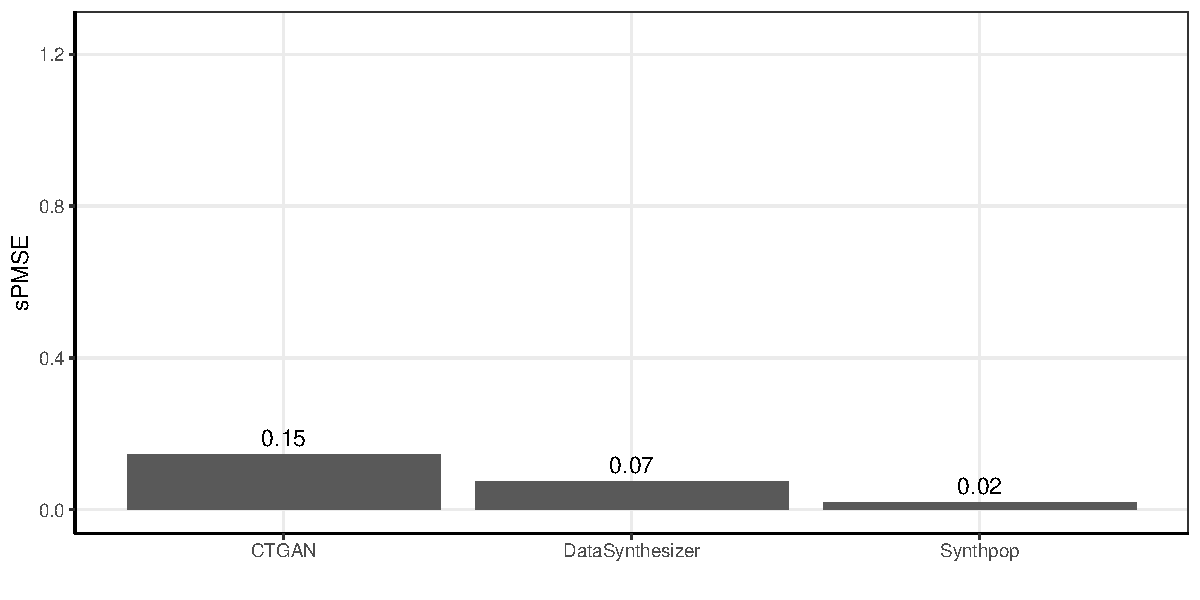
\includegraphics{../graphs/graph_fidelity_compare_dataset.pdf}}
        \label{subfig:graph_fidelity_compare_dataset}
    \end{subfigure}

    \begin{subfigure}{\textwidth}
        \caption{Two-way pMSE}
        \resizebox{\textwidth}{!}{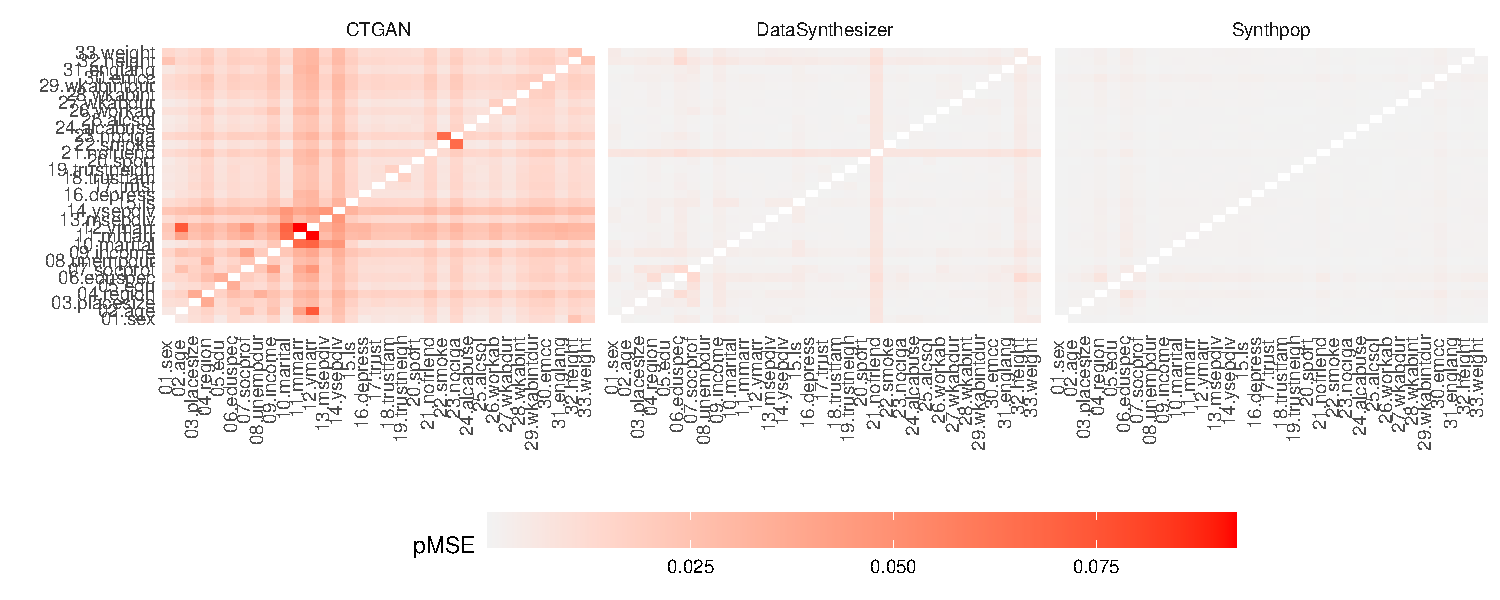
\includegraphics{../graphs/graph_fidelity_twoway_compare.pdf}}
        \label{subfig:graph_fidelity_compare_twoway}
    \end{subfigure}
\end{figure}


\begin{figure}[ht]
    \caption{Comparing one-way frequency of select variables and ROE}
    \label{fig:graph_frequency_compare}
    \centering

    \begin{subfigure}{\textwidth}
        \centering        
        \caption{Number of friends}
        \resizebox{.9\textwidth}{!}{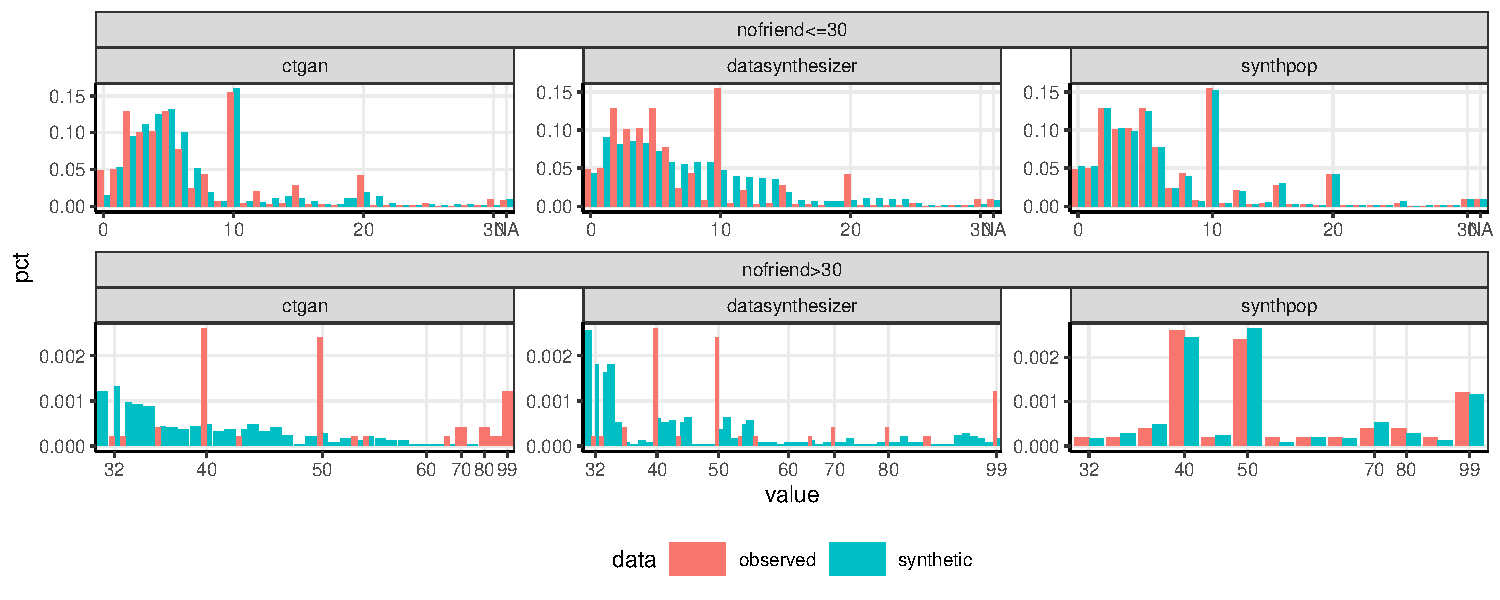
\includegraphics{../graphs/compare_nofriend_1.pdf}}
        \label{subfig:graph_frequency_compare_nofriend}
    \end{subfigure}

    \begin{subfigure}{\textwidth}
        \centering        
        \caption{BMI}
        \resizebox{.9\textwidth}{!}{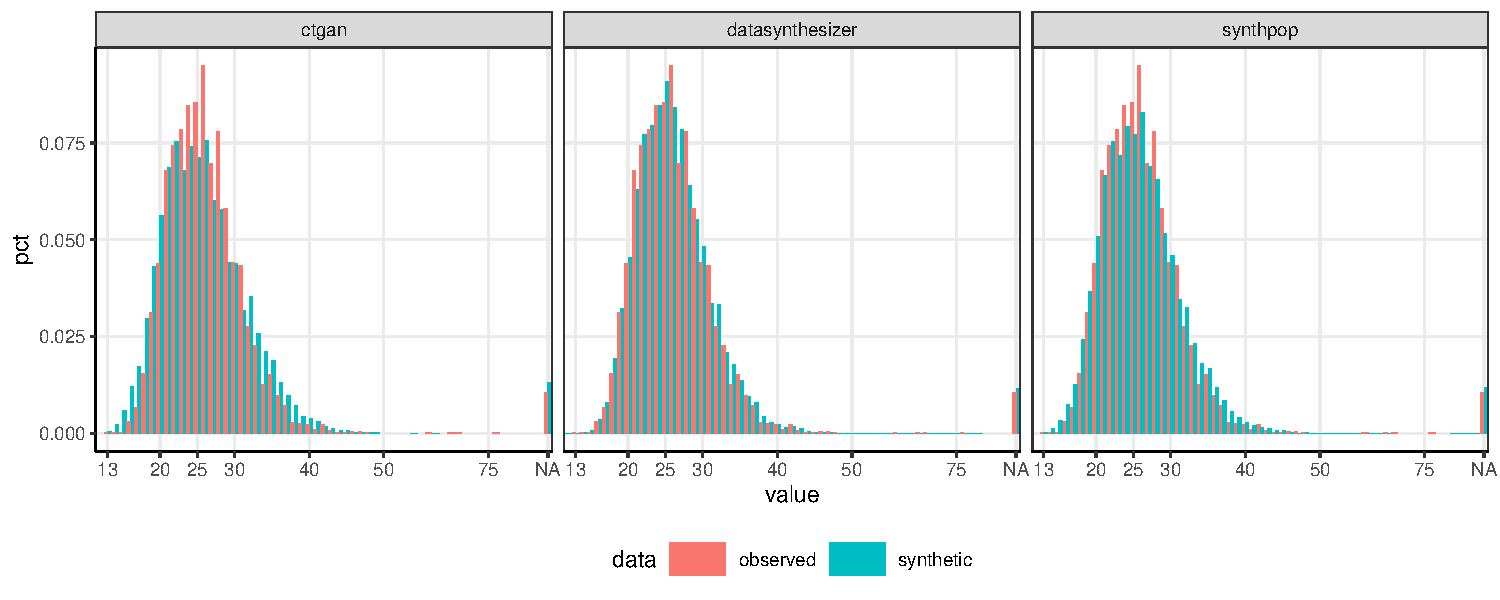
\includegraphics{../graphs/compare_bmi_1.pdf}}
        \label{subfig:graph_frequency_compare_bmi}
    \end{subfigure}

    \begin{subfigure}{\textwidth}
        \centering        
        \caption{Work abroad duration}
        \resizebox{.9\textwidth}{!}{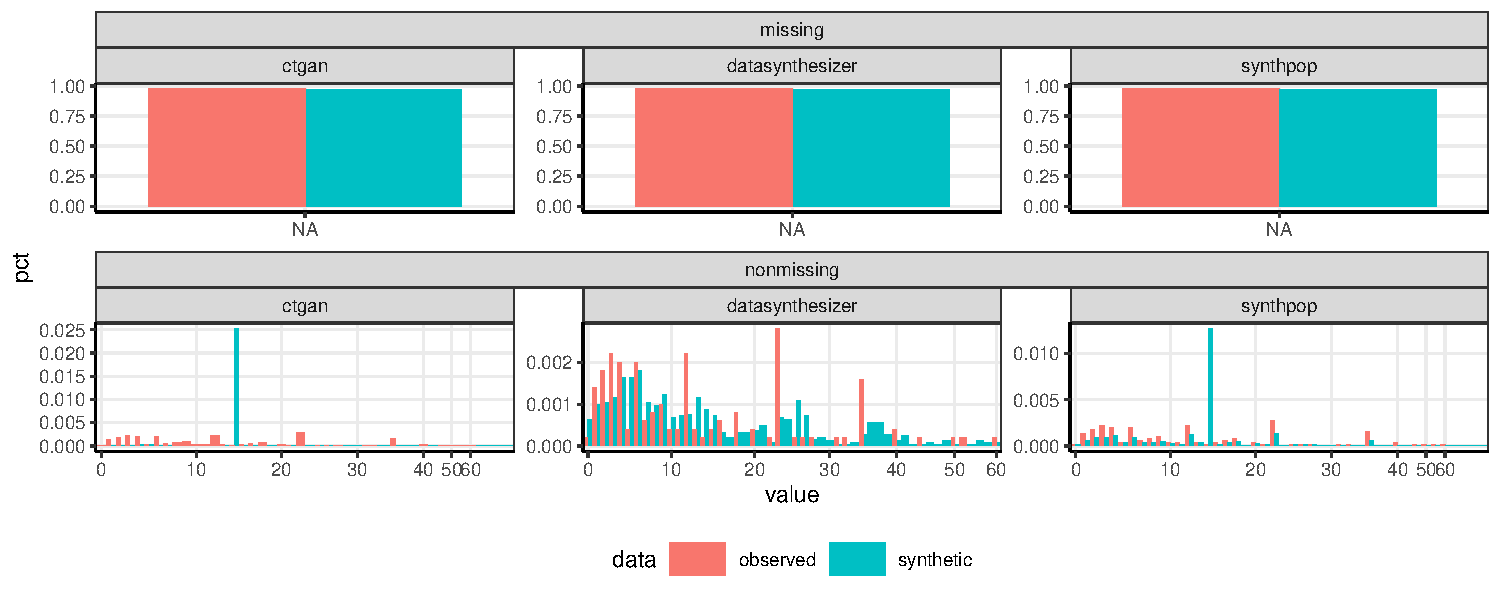
\includegraphics{../graphs/compare_wkabdur_1.pdf}}
        \label{subfig:graph_frequency_compare_wkabdur}
    \end{subfigure}

    \begin{subfigure}{\textwidth}
        \centering        
        \caption{Ratio of estimates (ROE)}
        \resizebox{.9\textwidth}{!}{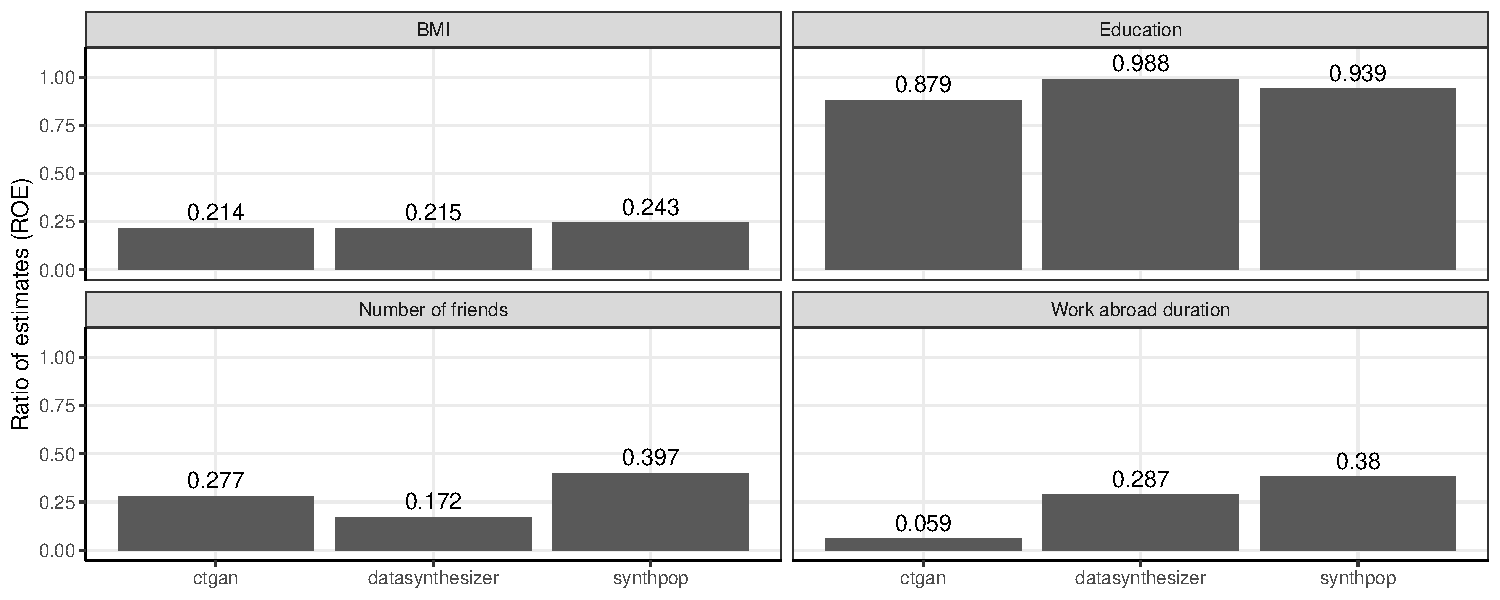
\includegraphics{../graphs/graph_compare_roe.pdf}}
        \label{subfig:graph_compare_roe}
    \end{subfigure}
\end{figure}

\begin{figure}
    \caption{Confidence interval overlap}
    \resizebox{\textwidth}{!}{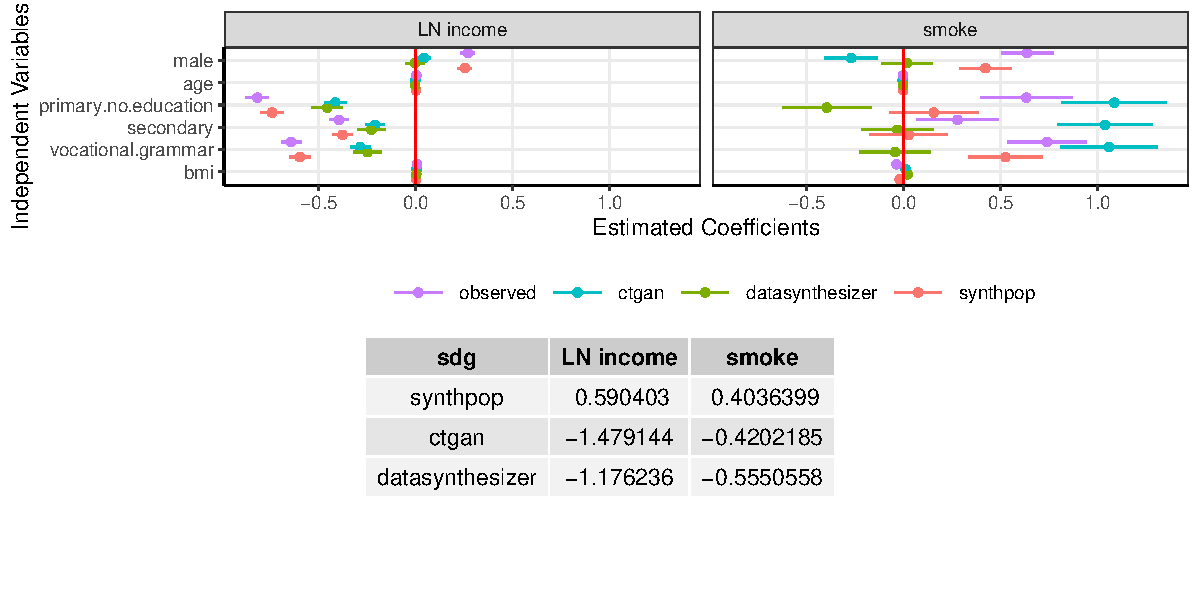
\includegraphics{../graphs/graph_utility_regression_cio_both.pdf}}
    \label{fig:utility_compare_cio}
\end{figure}


%%%%%%%%%%%%%%%%%%%%%%%%%%%%%%%%
% Bibliography
%%%%%%%%%%%%%%%%%%%%%%%%%%%%%%%%
\clearpage
\bibliographystyle{splncs04}
\bibliography{references}

%%%%%%%%%%%%%%%%%%%%%%%%%%%%%%%%
% Appendix
%%%%%%%%%%%%%%%%%%%%%%%%%%%%%%%%
\clearpage
\appendix
%%%%%%%%%%%%%%%%%%%%%%%%%%%%%%%%%%%%%%
%%%%%%%%%%%%%%%%%%%%%%%%%%%%%%%%%%%%%%
%Table
%%%%%%%%%%%%%%%%%%%%%%%%%%%%%%%%%%%%%%
%%%%%%%%%%%%%%%%%%%%%%%%%%%%%%%%%%%%%%

% \begin{table}[ht]
%     \caption{Versions of Social Diagnosis 2011 (SD2011)}
%     \centering
%     % latex table generated in R 4.3.0 by xtable 1.8-4 package
% Thu Feb  1 15:54:24 2024
\begin{tabular}{lll}
    \toprule
Data & & Description \\ \midrule
SD2011(a) && Raw data \\
SD2011(b) && + Cleaned: Missings are numeric values $<$ 0 and empty categorical cells \\
SD2011(c) && + Drop generated variables (\texttt{bmi} and \texttt{agegr}) \\
    \bottomrule
\end{tabular}

%     \label{table:sd2011_versions}
% \end{table}


%%%%%%%%%%%%%%%%%%%%%%%%%%%%%%%%%%%%%%
% Appendix
% DATASYNTHESIZER
%%%%%%%%%%%%%%%%%%%%%%%%%%%%%%%%%%%%%%
\section{Appendix: DataSynthesizer}\label{appendix:datasynethsizer}
\setcounter{figure}{0}    
\setcounter{table}{0}    
\renewcommand*\thetable{\Alph{section}.\arabic{table}}
\renewcommand*\thefigure{\Alph{section}.\arabic{figure}}
\renewcommand{\theHfigure}{\Alph{section}.\arabic{table}}
\renewcommand{\theHtable}{\Alph{section}.\arabic{figure}}

\begin{figure}[ht]
  \caption{Tuning DataSynthesizer across parents}
  \label{fig:tuning_ds}
  \centering
  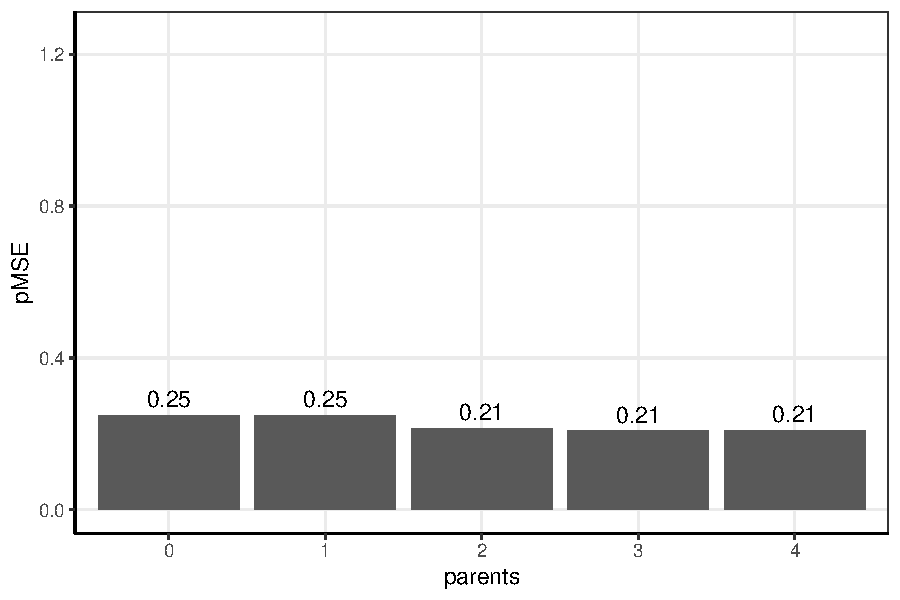
\includegraphics[width=\linewidth]{../graphs/datasynthesizer/datasynthesizer_fidelity_optimize_dataset_parents.pdf}
  \label{fig:tuning_ds_dataset}
\end{figure}

\begin{figure}[ht]
  \caption{Datasynthesizer two-way correlation  (pMSE)}
  \label{fig:ds_fidelity_two_way}
  \centering

  \begin{subfigure}{0.75\textwidth}
    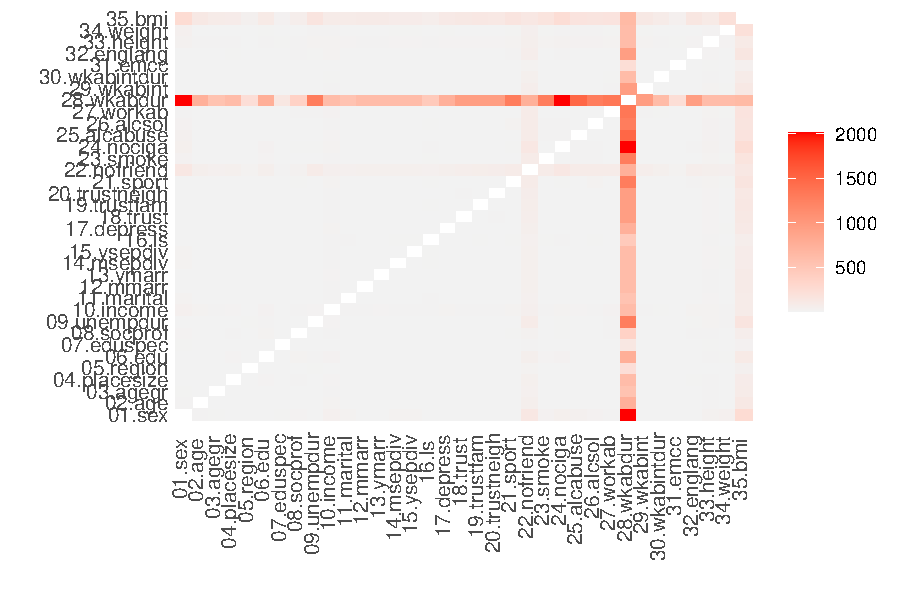
\includegraphics[width=\linewidth]{../graphs/datasynthesizer/datasynthesizer_fidelity_twoway_sd2011.pdf}
    \caption{SD2011(a)}
    \label{subfig:ds_fidelity_two_way_subfig-a}
  \end{subfigure}

  \begin{subfigure}{0.75\textwidth}
    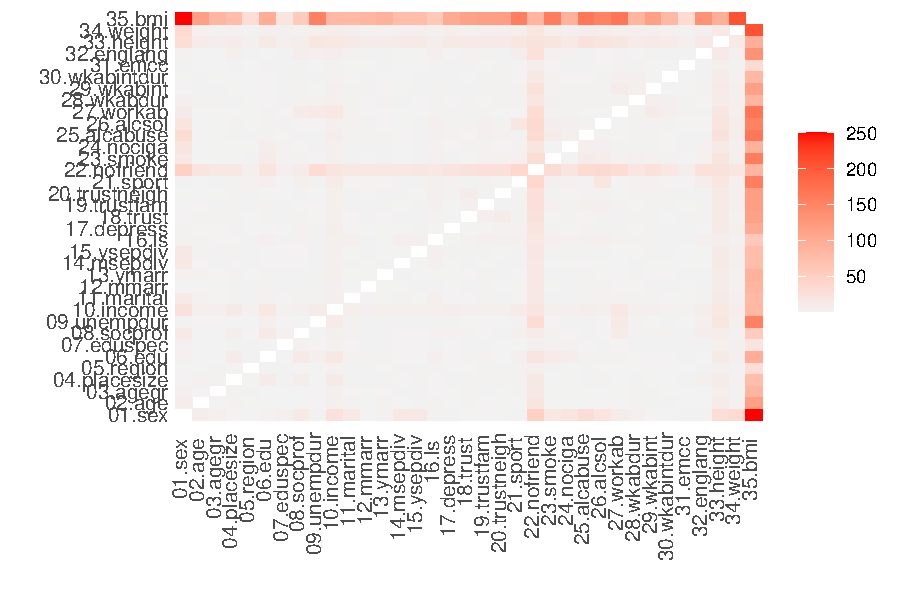
\includegraphics[width=\linewidth]{../graphs/datasynthesizer/datasynthesizer_fidelity_twoway_sd2011_clean.pdf}
    \caption{SD2011(b)}
    \label{subfig:ds_fidelity_two_way_subfig-b}
  \end{subfigure}

  \begin{subfigure}{0.75\textwidth}
    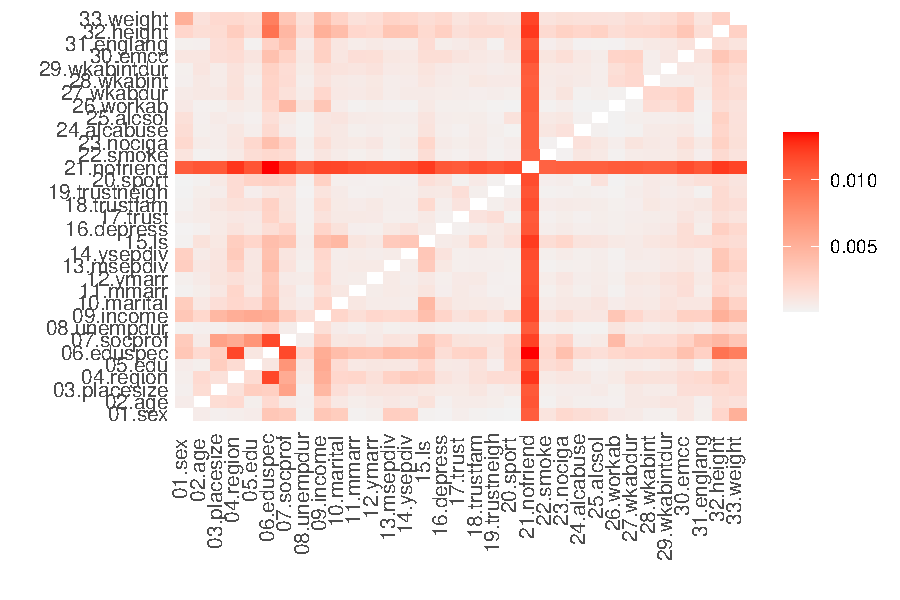
\includegraphics[width=\linewidth]{../graphs/datasynthesizer/datasynthesizer_fidelity_twoway_sd2011_clean_small.pdf}
    \caption{SD2011(c)}
    \label{subfig:ds_fidelity_two_way_subfig-c}
  \end{subfigure}
\end{figure}

\begin{figure}[ht]
  \caption{Frequency values for original and synthetic data (DataSynthesizer)}
  \label{fig:ds_variables}
  \centering

\begin{subfigure}{\textwidth}
    \caption{Variable: \texttt{wkabdur} (Work abroad duration)}
    \resizebox{\textwidth}{!}{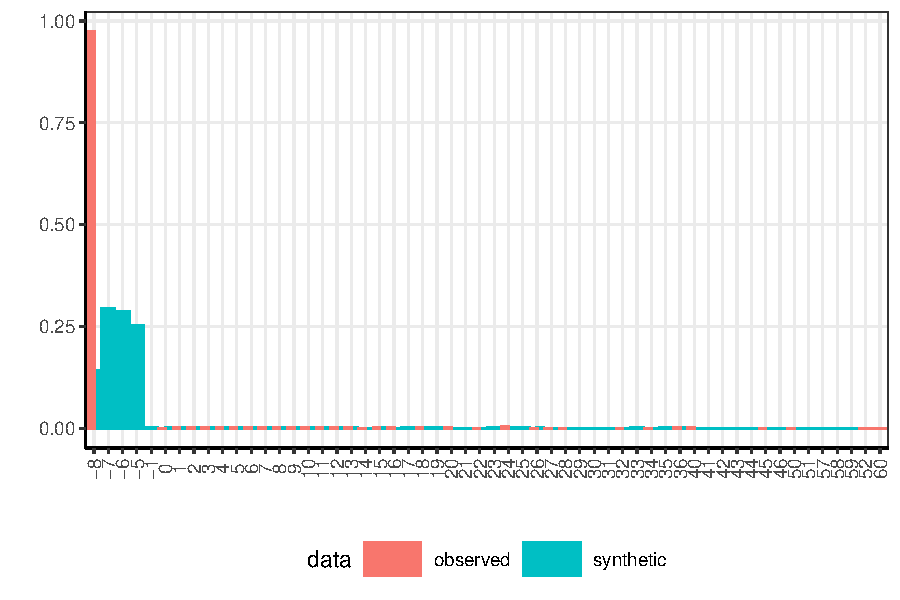
\includegraphics{../graphs/datasynthesizer/datasynthesizer_wkabdur.pdf}}
    \label{subfig:ds_variable_wkabdur}
\end{subfigure}

\begin{subfigure}{\textwidth}
    \caption{Variable: \texttt{bmi} (Body mass index)}
    \resizebox{\textwidth}{!}{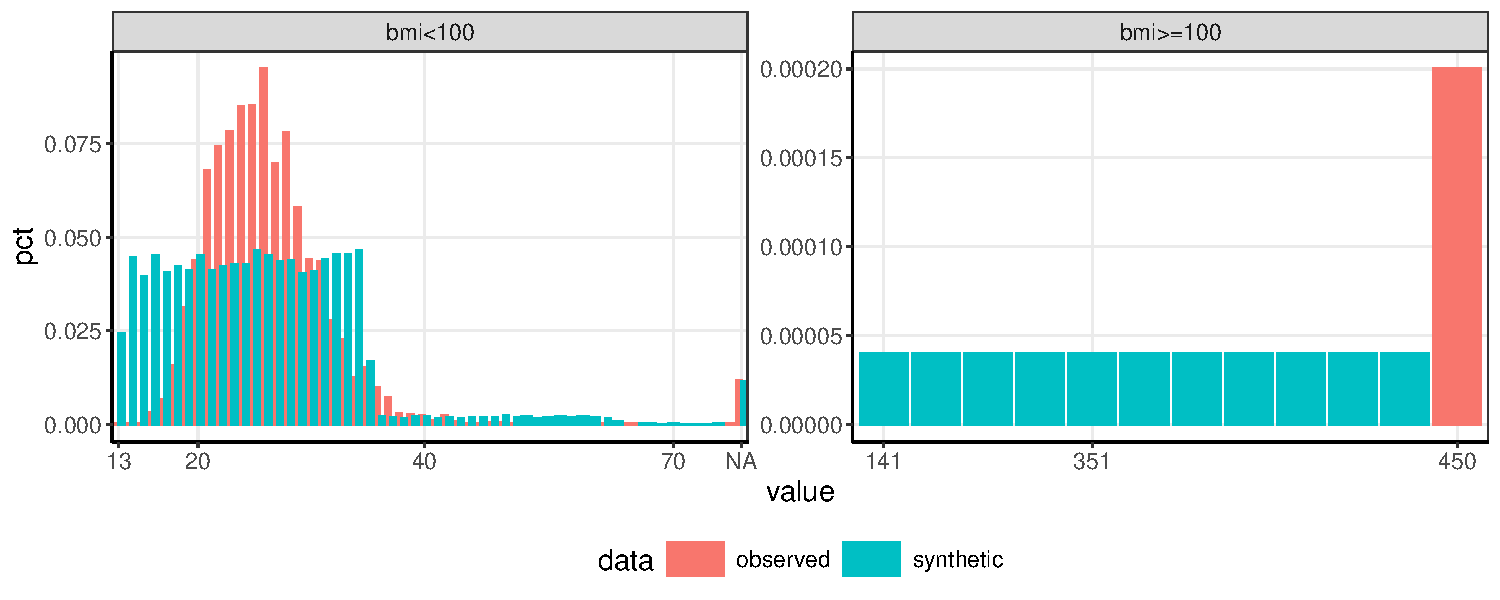
\includegraphics{../graphs/datasynthesizer/datasynthesizer_bmi.pdf}}
    \label{subfig:ds_variable_bmi}
\end{subfigure}


\begin{subfigure}{\textwidth}
    \caption{Variable: \texttt{nofriend} (Number of friends)}
    \resizebox{\textwidth}{!}{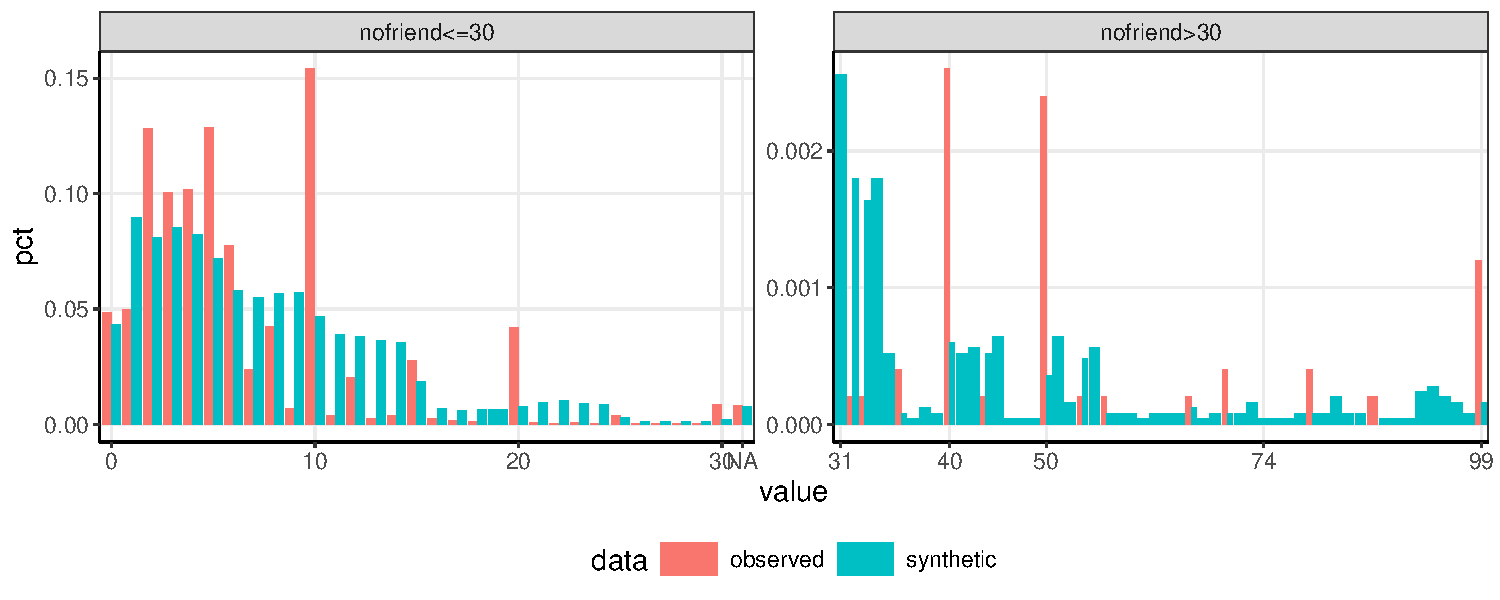
\includegraphics{../graphs/datasynthesizer/datasynthesizer_nofriend.pdf}}
    \label{subfig:ds_variable_nofriend}
\end{subfigure}
\end{figure}

\begin{figure}[ht]
  \caption{Tuning DataSynthesizer across data sets (parents = 2)}
  \label{fig:tuning_ds}
  \centering
  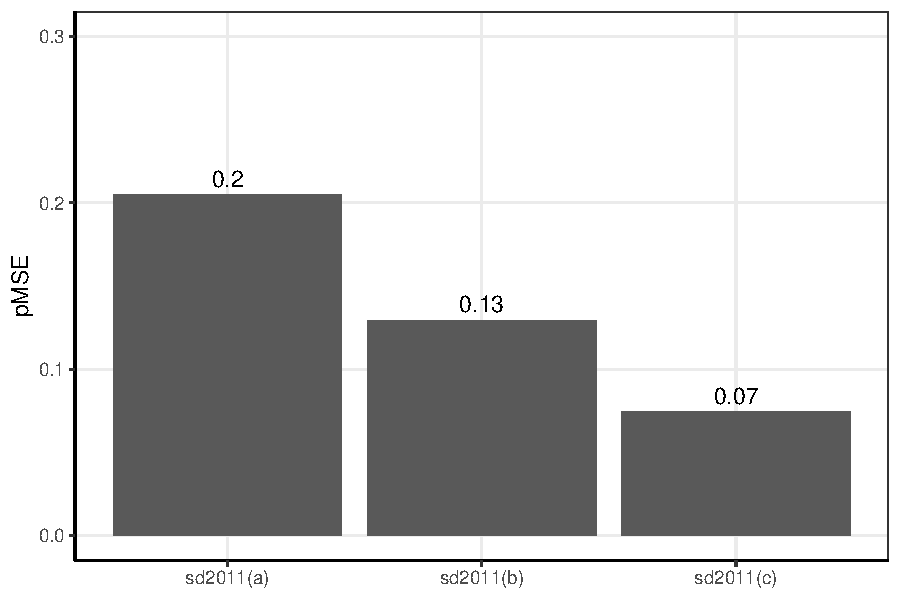
\includegraphics[width=\linewidth]{../graphs/datasynthesizer/datasynthesizer_fidelity_optimize_dataset_compare.pdf}
  \label{fig:tuning_ds_optimize_dataset_compare}
\end{figure}


%%%%%%%%%%%%%%%%%%%%%%%%%%%%%%%%%%%%%%
% Appendix
% CTGAN
%%%%%%%%%%%%%%%%%%%%%%%%%%%%%%%%%%%%%%
\clearpage
\section{Appendix: CTGAN}\label{appendix:CTGAN}
\setcounter{figure}{0}    
\setcounter{table}{0}    
\renewcommand*\thetable{\Alph{section}.\arabic{table}}
\renewcommand*\thefigure{\Alph{section}.\arabic{figure}}
\renewcommand{\theHfigure}{\Alph{section}.\arabic{table}}
\renewcommand{\theHtable}{\Alph{section}.\arabic{figure}}

\begin{table}[!h]
    \rowcolors{1}{white}{lightgray}
    \caption{Batch size and epochs = total steps}
    \centering
    \begin{tabular}{cllll>{\cellcolor{white}}p{1in}}
    % {cllllp{1in}}
    \toprule
    N & Batch size & Steps per Epoch & Epochs & Total Steps & Compare \\
    \midrule
    5.000 & 500 & 10 & 100 & 1,000 & \multirow{4}{1in}{Constant batch size, as shown in figure \ref{subfig:ctgan_fidelity_optimize_batch_size}}\\
    5.000 & 500 & 10 & 300 & 3,000 \\
    5.000 & 500 & 10 & 600 & 6,000 \\
    5.000 & 500 & 10 & 900 & 9,000 \\ \hline
    5.000 & 100 & 50 & 60 & 3,000  & \multirow{4}{1in}{Constant batch size, as shown in figure \ref{subfig:ctgan_fidelity_optimize_epochs}} \\
    5.000 & 250 & 20 & 150 & 3,000 \\
    5.000 & 500 & 10 & 300 & 3,000 \\
    5.000 & 1.000 & 5 & 600 & 3,000 \\ 
    \bottomrule
    \end{tabular}
\end{table}

\begin{figure}[ht]
  \caption{Tuning CTGAN (effect of steps)}
  \label{fig:ctgan_fidelity_optimize}
  \centering

  \begin{subfigure}{0.75\textwidth}
  \caption{Effect of batch size with constant steps (3.000)}
  \resizebox{\textwidth}{!}{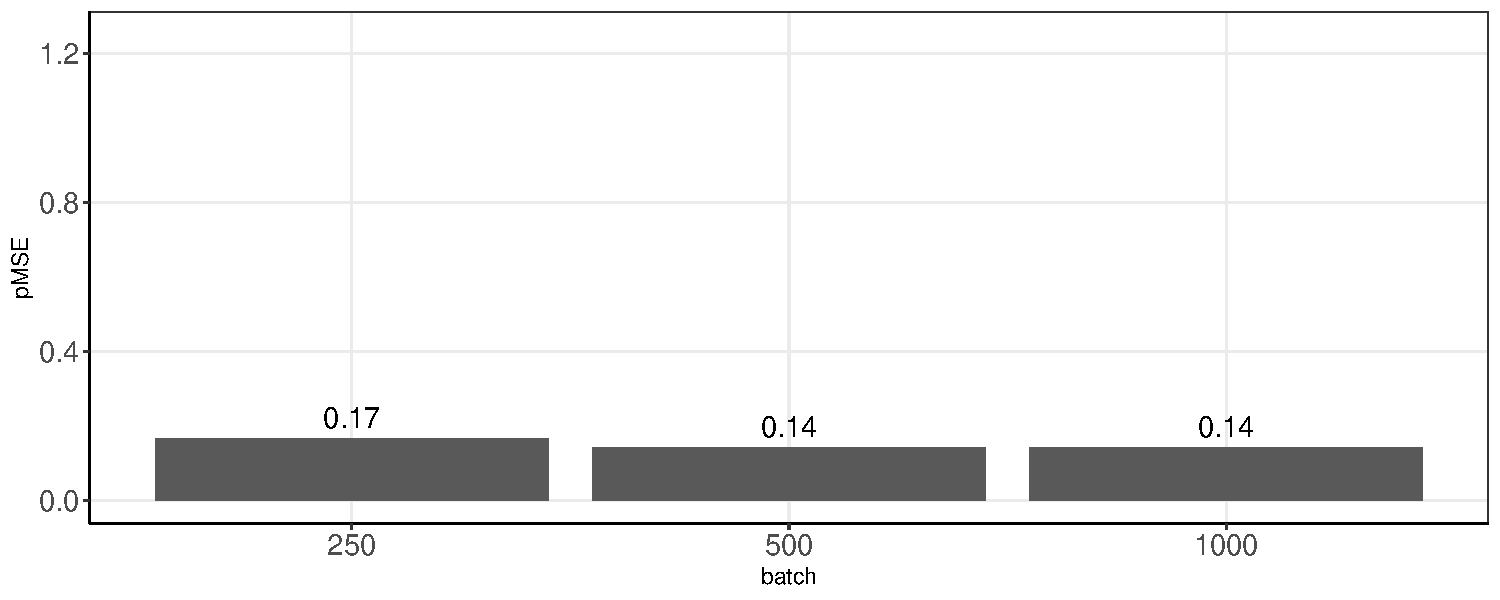
\includegraphics{../../ctgan/graphs/ctgan/ctgan_fidelity_optimize_batch_size.pdf}}
  \label{subfig:ctgan_fidelity_optimize_batch_size}
  \end{subfigure}

  \begin{subfigure}{0.75\textwidth}
  \caption{Effect of epoch number with constant batch size (500)}
  \resizebox{\textwidth}{!}{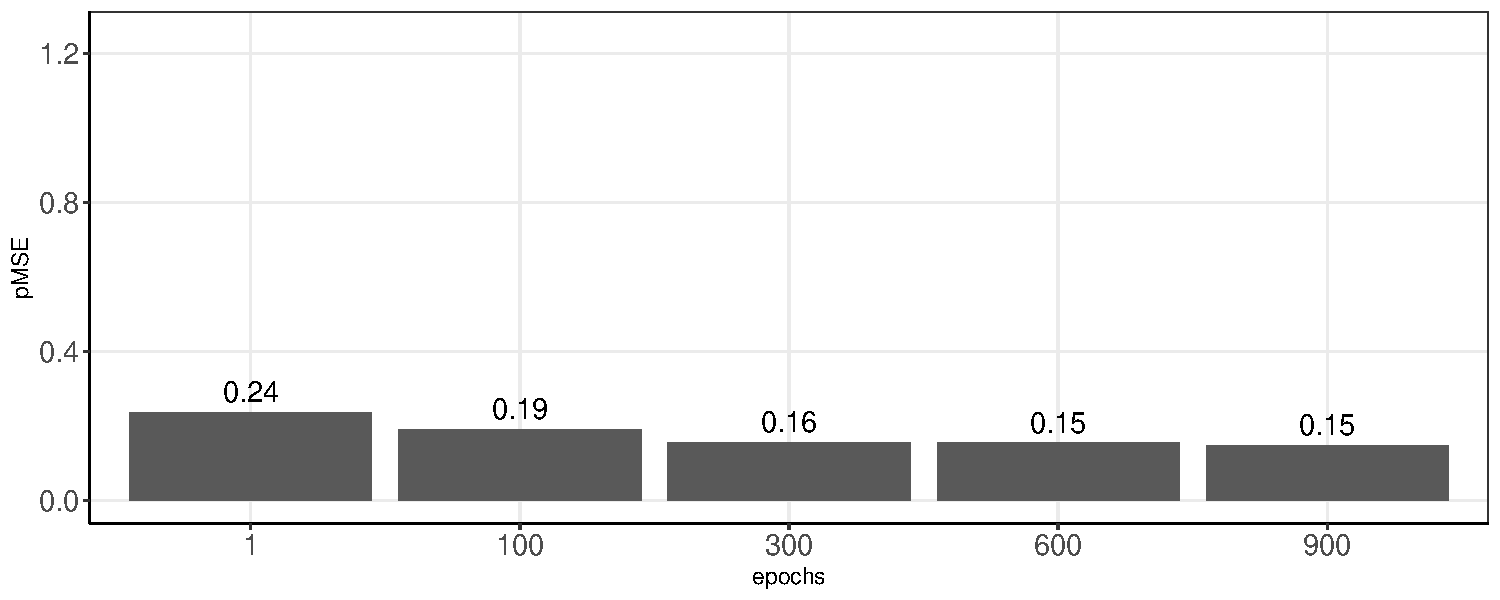
\includegraphics{../../ctgan/graphs/ctgan/ctgan_fidelity_optimize_epochs.pdf}}
  \label{subfig:ctgan_fidelity_optimize_epochs}
  \end{subfigure}

  \begin{subfigure}{0.75\textwidth}
    \caption{Effect of dimensionality}
      \resizebox{\textwidth}{!}{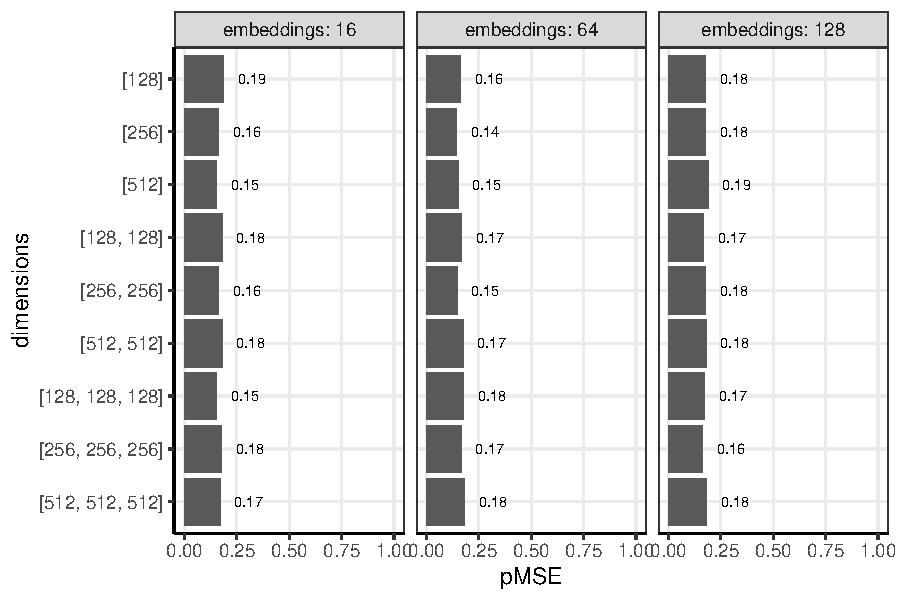
\includegraphics{../../ctgan/graphs/ctgan/ctgan_fidelity_optimize_dimensions.pdf}}
      \label{subfig:ctgan_fidelity_optimize_dimensions}
  \end{subfigure}
\end{figure}


\begin{figure}[ht]
  \caption{CTGAN two-way correlation (pMSE)}
  \label{fig:ctgan_fidelity_two_way}
  \centering

  \begin{subfigure}{0.75\textwidth}
    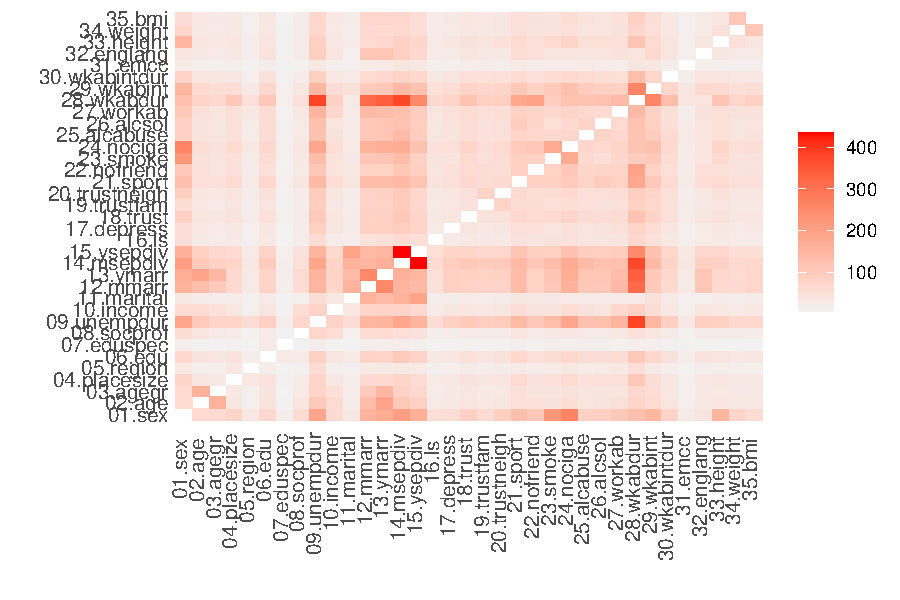
\includegraphics[width=\linewidth]{../graphs/ctgan/ctgan_fidelity_twoway_sd2011.pdf}
    \caption{SD2011(a)}
    \label{fig:ctgan_fidelity_two_way_subfig-a}
  \end{subfigure}

  \begin{subfigure}{0.75\textwidth}
    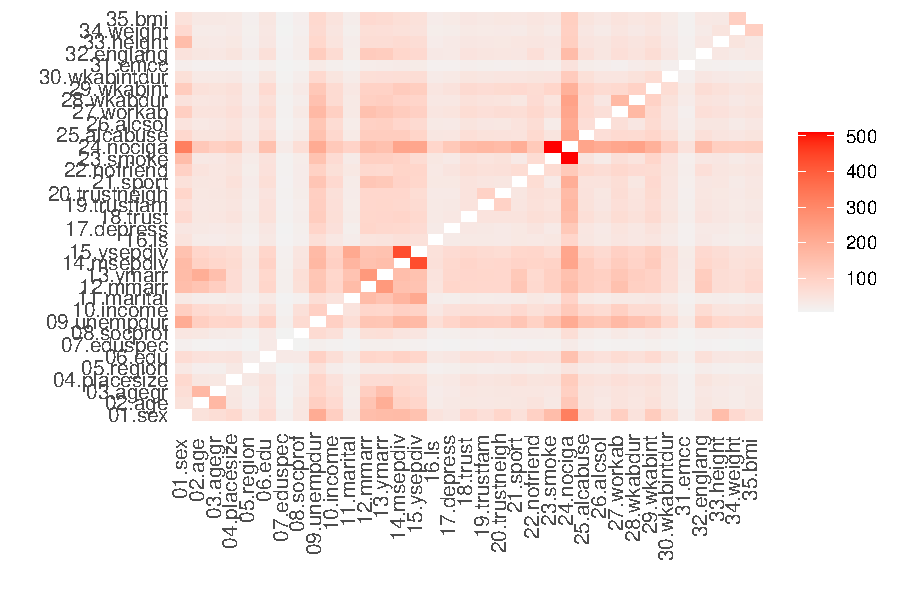
\includegraphics[width=\linewidth]{../graphs/ctgan/ctgan_fidelity_twoway_sd2011_clean.pdf}
    \caption{SD2011(b)}
    \label{fig:ctgan_fidelity_two_way_subfig-b}
  \end{subfigure}

  \begin{subfigure}{0.75\textwidth}
    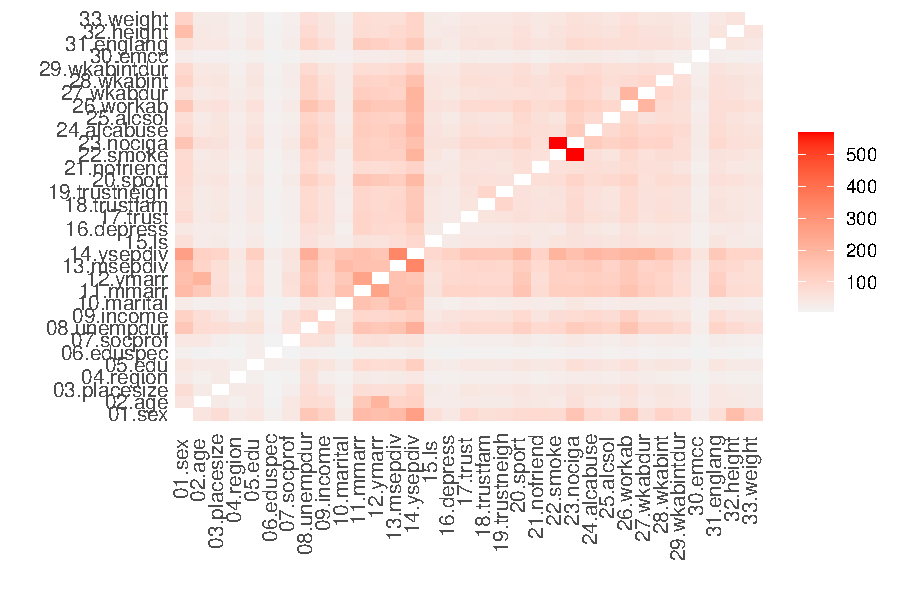
\includegraphics[width=\linewidth]{../graphs/ctgan/ctgan_fidelity_twoway_sd2011_clean_small.pdf}
    \caption{SD2011(c)}
    \label{fig:ctgan_fidelity_two_way_subfig-c}
  \end{subfigure}

\end{figure}

%%%%%%%%%%%%%%%%%%%%%%%%%%%%%%%%%%%%%%
%%%%%%%%%%%%%%%%%%%%%%%%%%%%%%%%%%%%%%
%SYNTHPOP
%%%%%%%%%%%%%%%%%%%%%%%%%%%%%%%%%%%%%%
%%%%%%%%%%%%%%%%%%%%%%%%%%%%%%%%%%%%%%
\begin{figure}[ht]
  \caption{Synthpop two-way correlation  (pMSE)}
  \label{fig:synthpop_fidelity_two_way}
  \centering

  \begin{subfigure}{0.75\textwidth}
    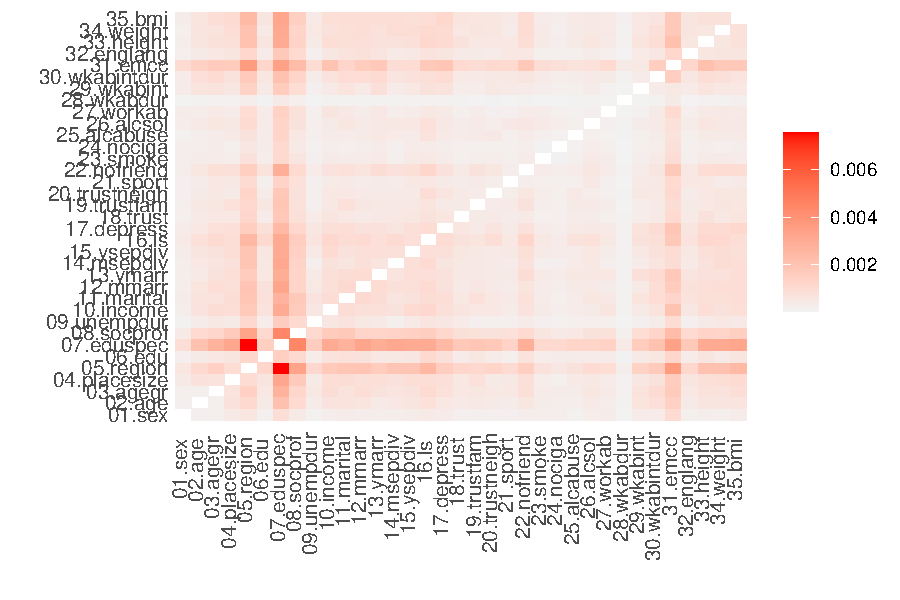
\includegraphics[width=\linewidth]{../graphs/synthpop/synthpop_fidelity_twoway_sd2011.pdf}
    \caption{SD2011(a)}
    \label{fig:synthpop_fidelity_two_way_subfig-a}
  \end{subfigure}

  \begin{subfigure}{0.75\textwidth}
    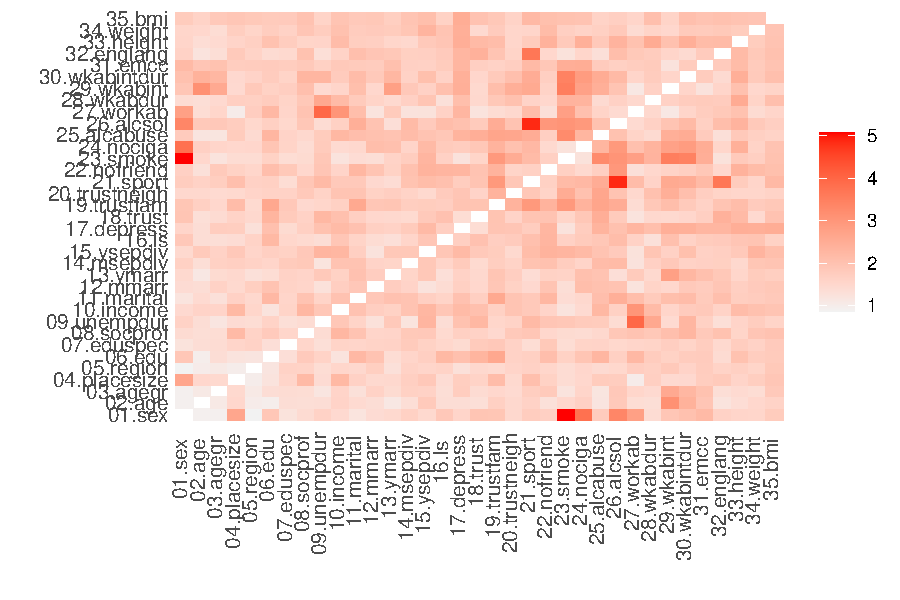
\includegraphics[width=\linewidth]{../graphs/synthpop/synthpop_fidelity_twoway_sd2011_clean.pdf}
    \caption{SD2011(b)}
    \label{fig:synthpop_fidelity_two_way_subfig-b}
  \end{subfigure}

  \begin{subfigure}{0.75\textwidth}
    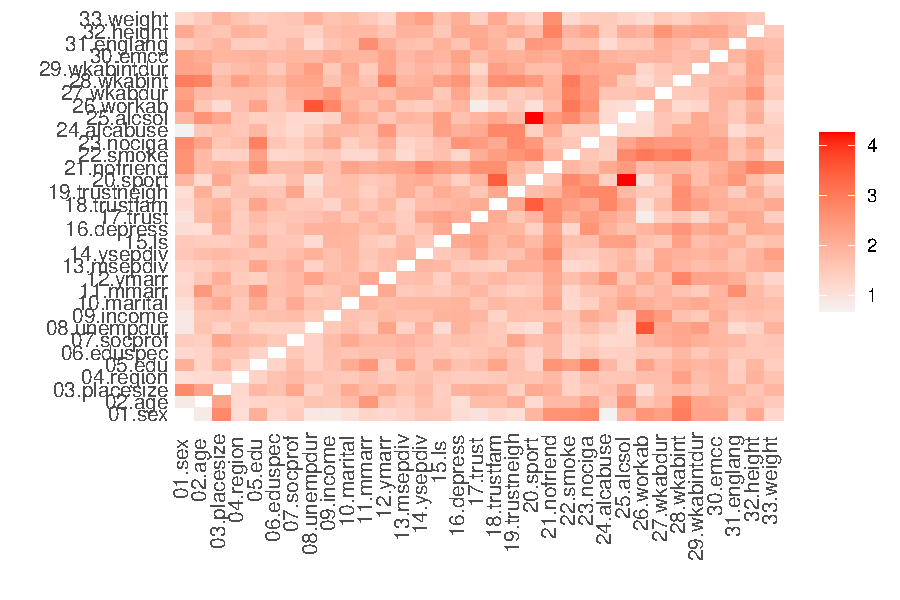
\includegraphics[width=\linewidth]{../graphs/synthpop/synthpop_fidelity_twoway_sd2011_clean_small.pdf}
    \caption{SD2011(c)}
    \label{fig:synthpop_fidelity_two_way_subfig-c}
  \end{subfigure}

\end{figure}



\end{document}
